% PsychoPy tutorial
% Ariel Rokem
% License:CC(http://creativecommons.org/licenses/by-nc-sa/3.0/)

\documentclass{beamer}

\usepackage{ulem}
\usepackage{listings,bera}

\usetheme{PaloAlto}
\beamertemplatenavigationsymbolsempty

\definecolor{fore}{RGB}{0,20,30}
\definecolor{back}{RGB}{255,255,255}
\definecolor{title}{RGB}{255,255,255}


\setbeamercolor{titlelike}{fg=title}
\setbeamercolor{normal text}{fg=fore,bg=back}
\definecolor{keywords}{RGB}{255,0,90}
\definecolor{comments}{RGB}{60,179,113}
\definecolor{strings}{RGB}{120,120,0}

\lstset{language=Python,
keywordstyle=\color{keywords},
commentstyle=\color{comments}\emph,
stringstyle=\color{strings}}

\title[nitime]{\tt{nitime}}
\subtitle
{Time-series analysis for fMRI data}

\author[Ariel Rokem] % (optional, use only with lots of authors)
{Ariel Rokem}
\date{June 3rd, 2011}
\institute[University of California, Berkeley]
{University of California, Berkeley}

\pgfdeclareimage[height=1.5cm]{ucb-logo}{figures/ucb_logo}
% put nipy logo in bottom left
\pgfdeclareimage[height=1.5cm]{nipper}{figures/nipper}
\setbeamertemplate{sidebar left}{
   \rlap{\hskip0.1cm%
     {\pgfuseimage{ucb-logo}}}
    \vfill%
   \rlap{\hskip0.1cm%
     {\pgfuseimage{nipper}}}%
   \vskip2pt%
   \llap{\usebeamertemplate***{navigation symbols}\hskip0.1cm}%
   \vskip2pt%
}

\begin{document}

%Title page:
\begin{frame}
  \titlepage
\end{frame}

\begin{frame}
\frametitle{The wiring diagram}
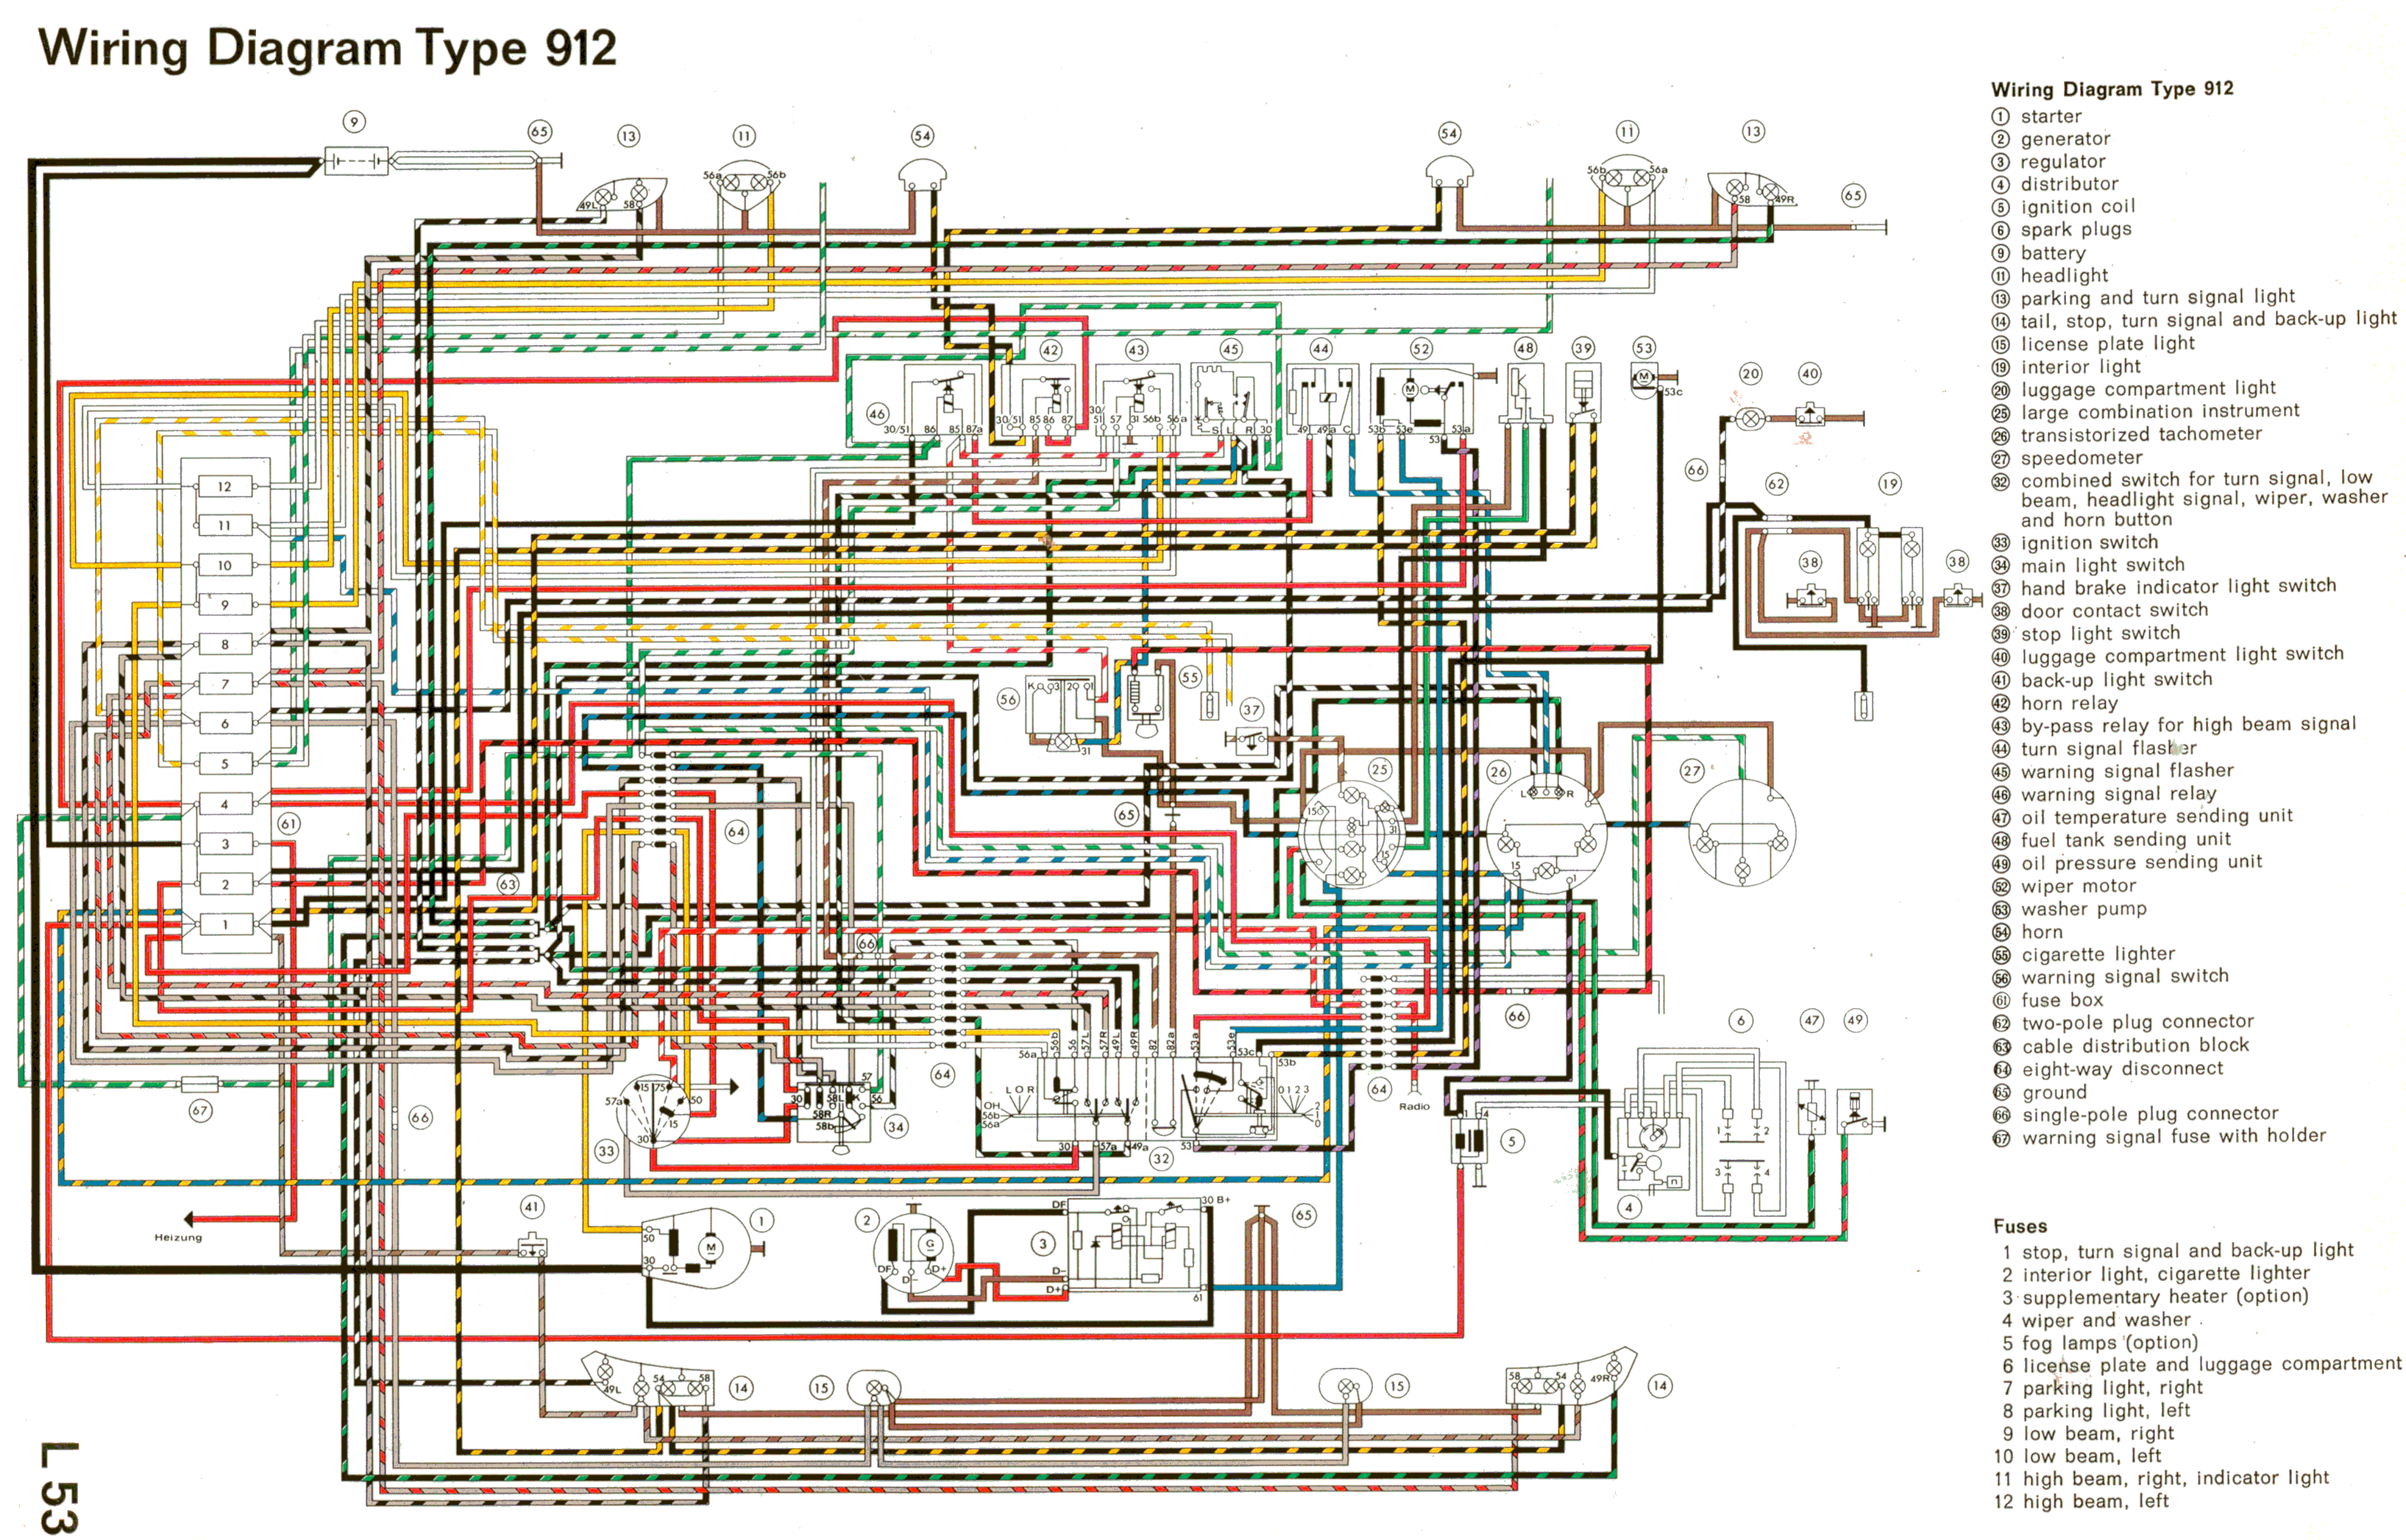
\includegraphics[height=5.7cm]{figures/wiring}
\end{frame}

\begin{frame}
\frametitle{The wiring diagram}
\includegraphics[height=5.7cm]{figures/felleman1}
\end{frame}

\begin{frame}
\frametitle{The wiring diagram}
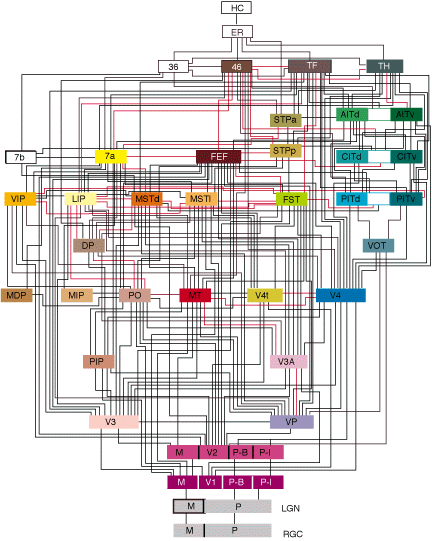
\includegraphics[height=5.7cm]{figures/felleman2}
\end{frame}

\begin{frame}
\frametitle{Task-specific networks}
  One of the goals of contemporary neuroscience is to delineate task-specific
  networks in the brain
\end{frame}

\begin{frame}
\frametitle{Time-series in fMRI data}
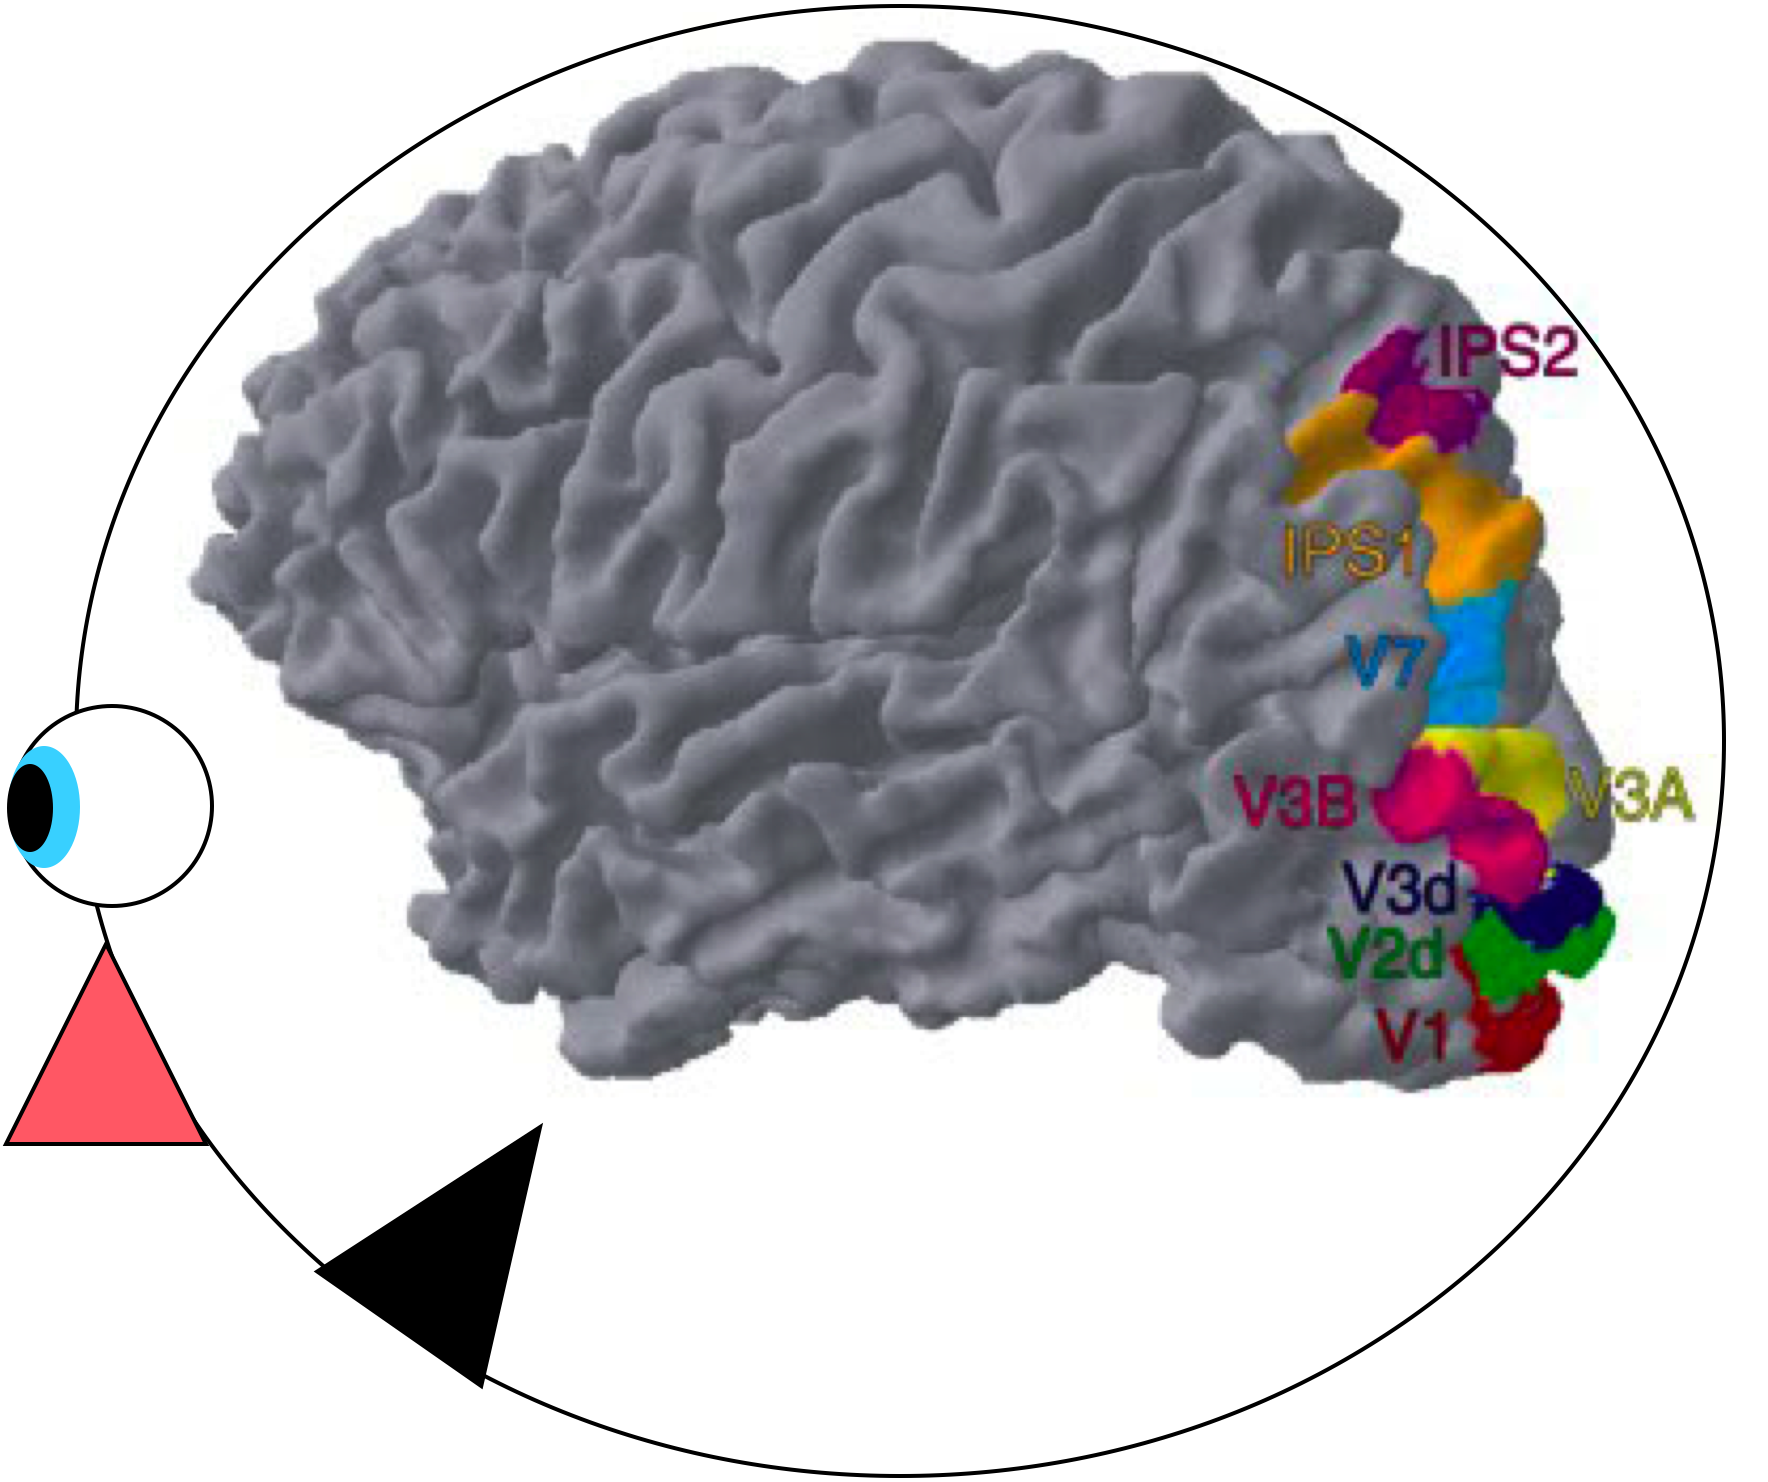
\includegraphics[height=5.7cm]{figures/brain_w_head}
\end{frame}

\begin{frame}
\frametitle{Time-series in fMRI data}
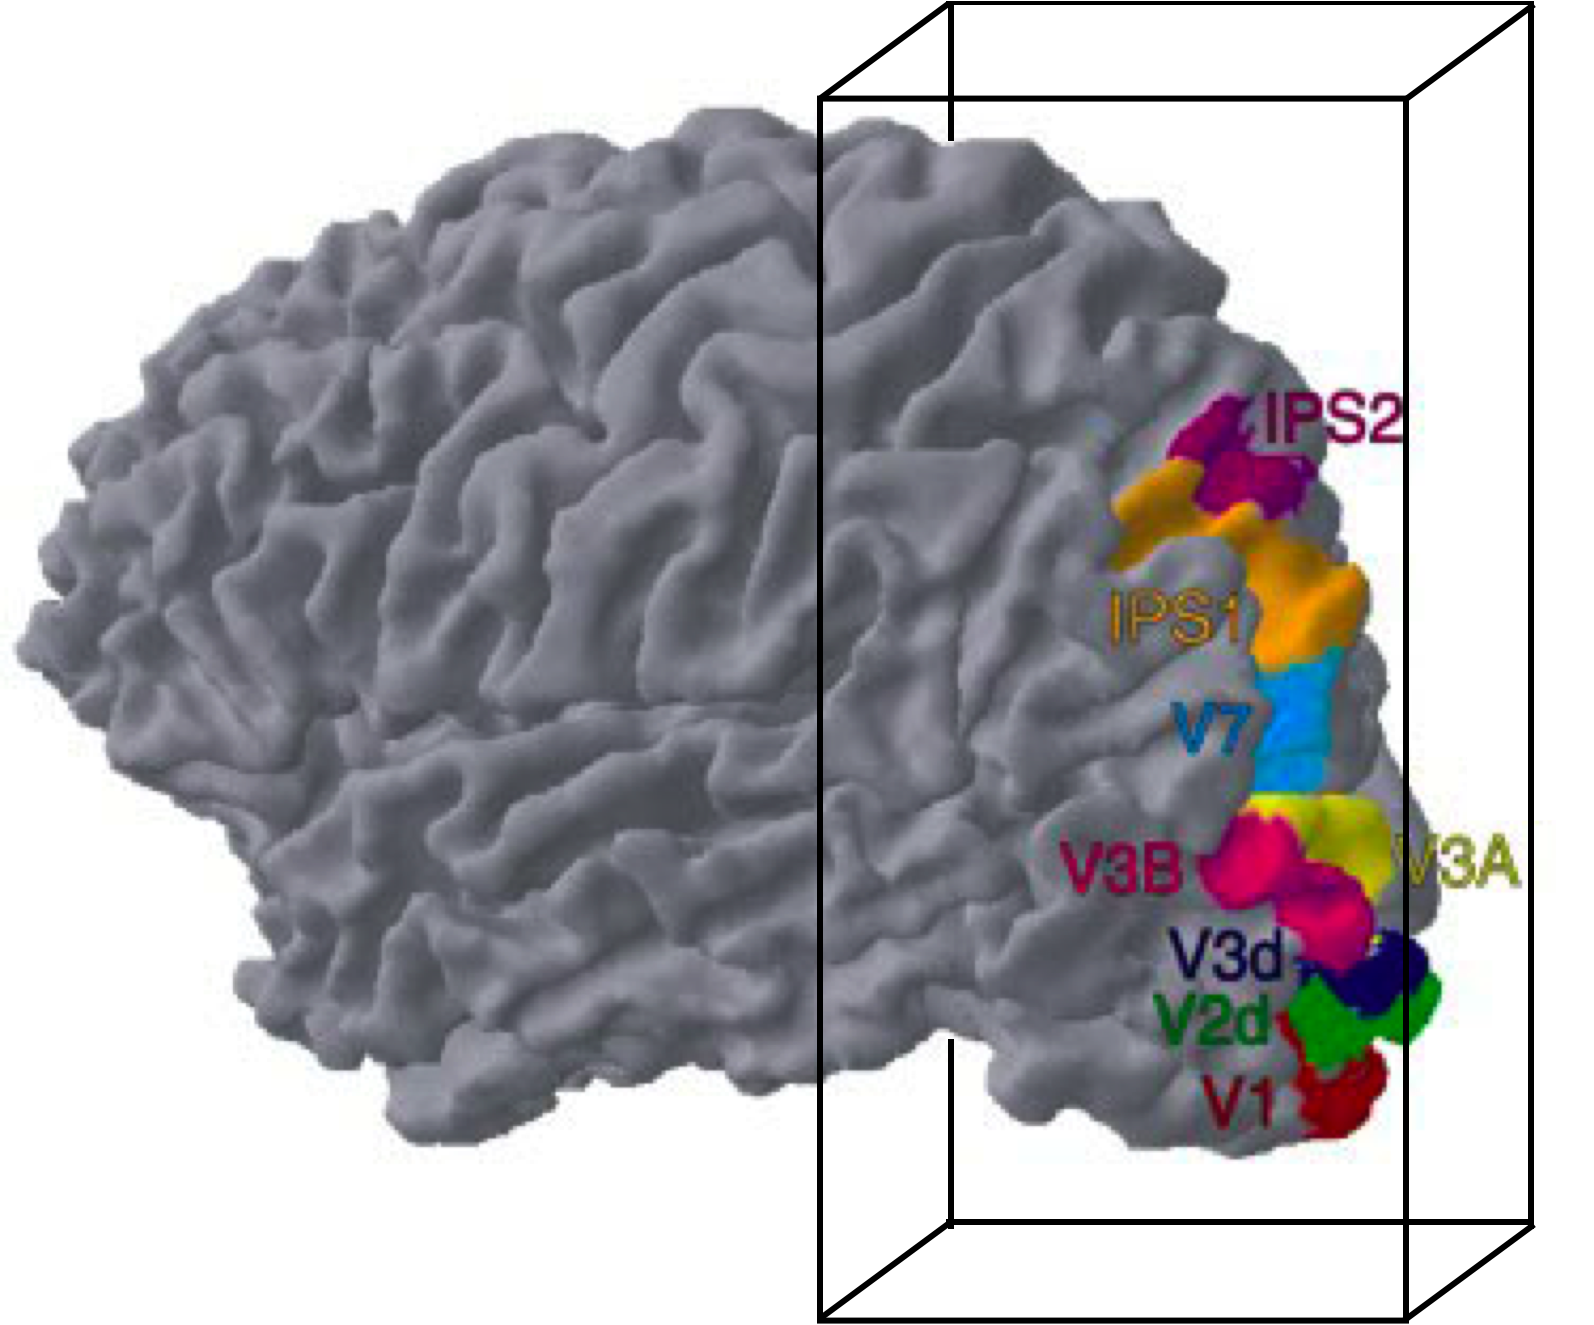
\includegraphics[height=5.7cm]{figures/brain_w_acquisition_vol}
\end{frame}

\begin{frame}
\frametitle{Time-series in fMRI data}
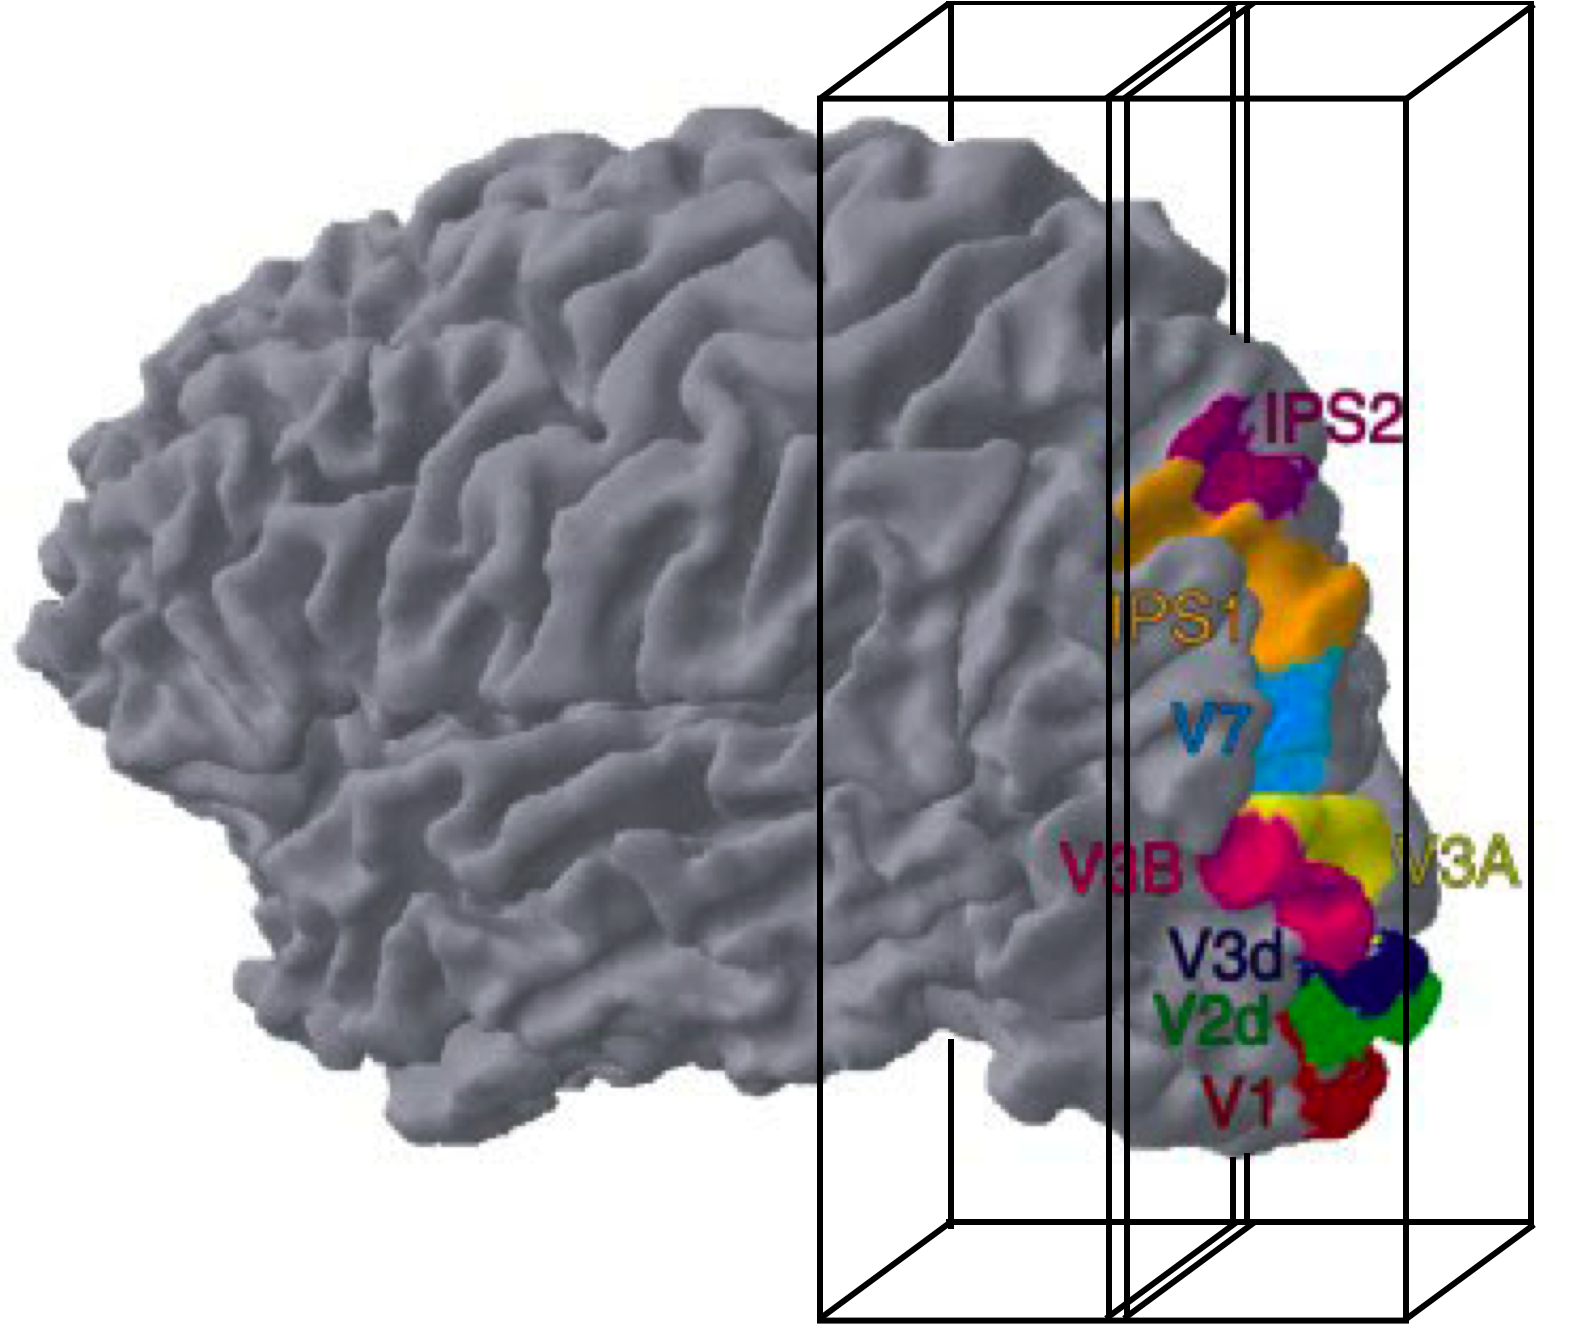
\includegraphics[height=5.7cm]{figures/brain_w_acquisition_vol_n_slice}
\end{frame}

\begin{frame}
\frametitle{Time-series in fMRI data}
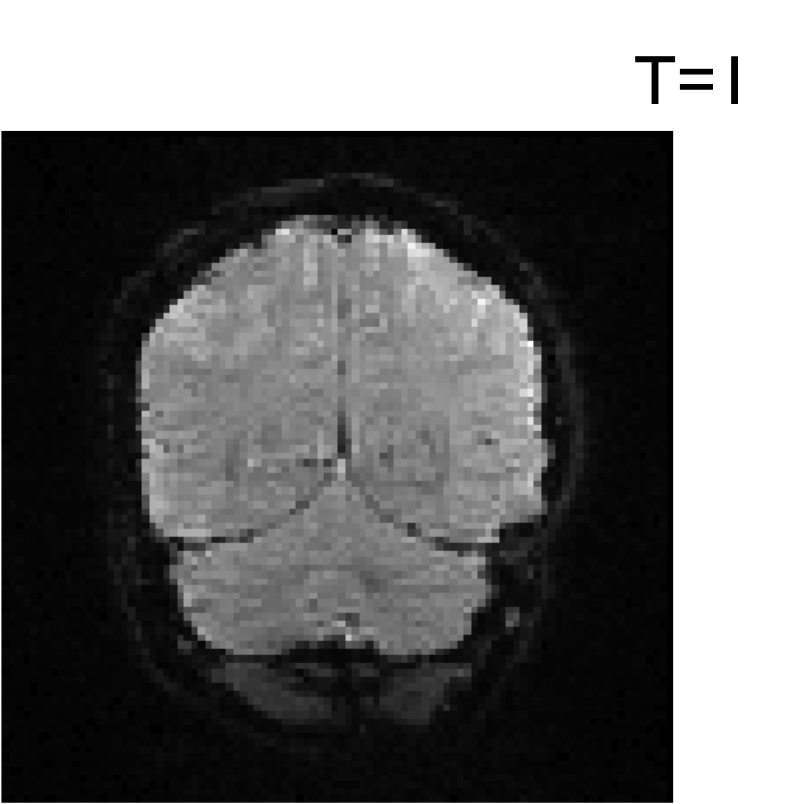
\includegraphics[height=5.7cm]{figures/t1}
\end{frame}

\begin{frame}
\frametitle{Time-series in fMRI data}
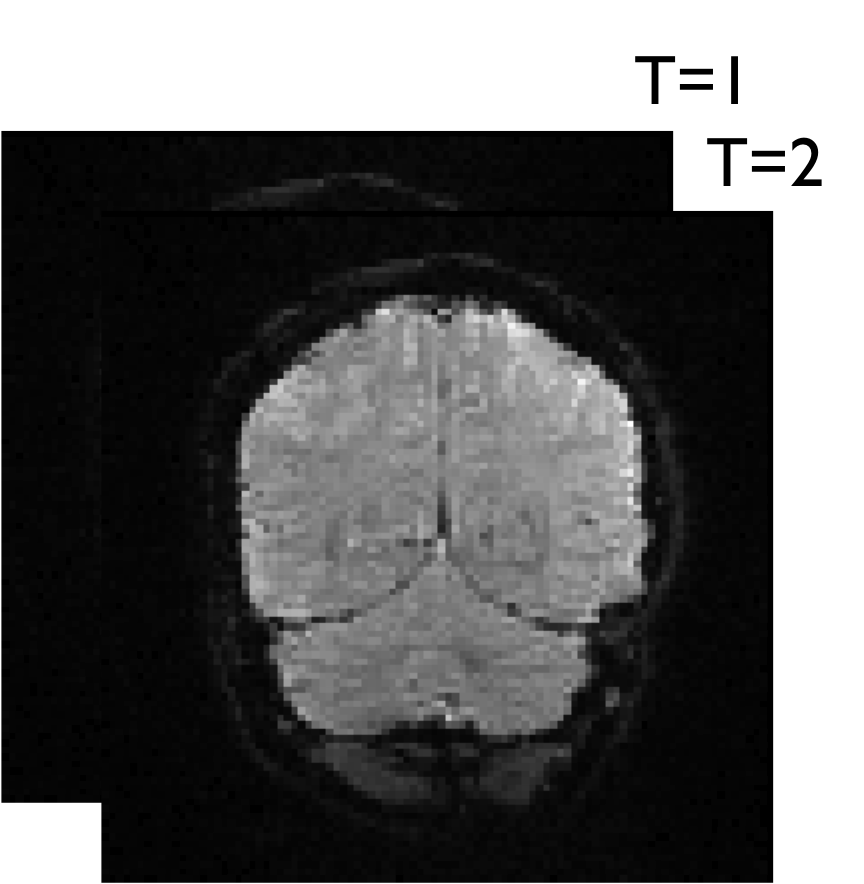
\includegraphics[height=5.7cm]{figures/t1_2}
\end{frame}

\begin{frame}
\frametitle{Time-series in fMRI data}
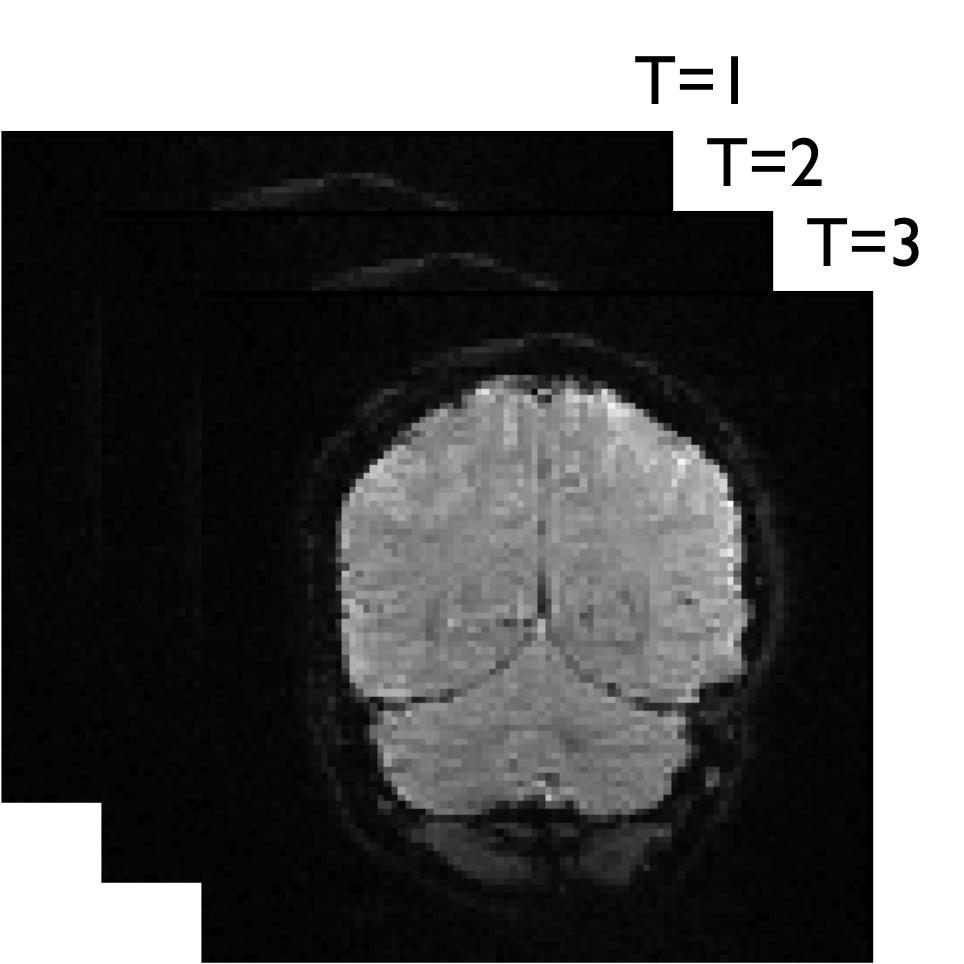
\includegraphics[height=5.7cm]{figures/t1_2_3}
\end{frame}

\begin{frame}
\frametitle{Time-series in fMRI data}
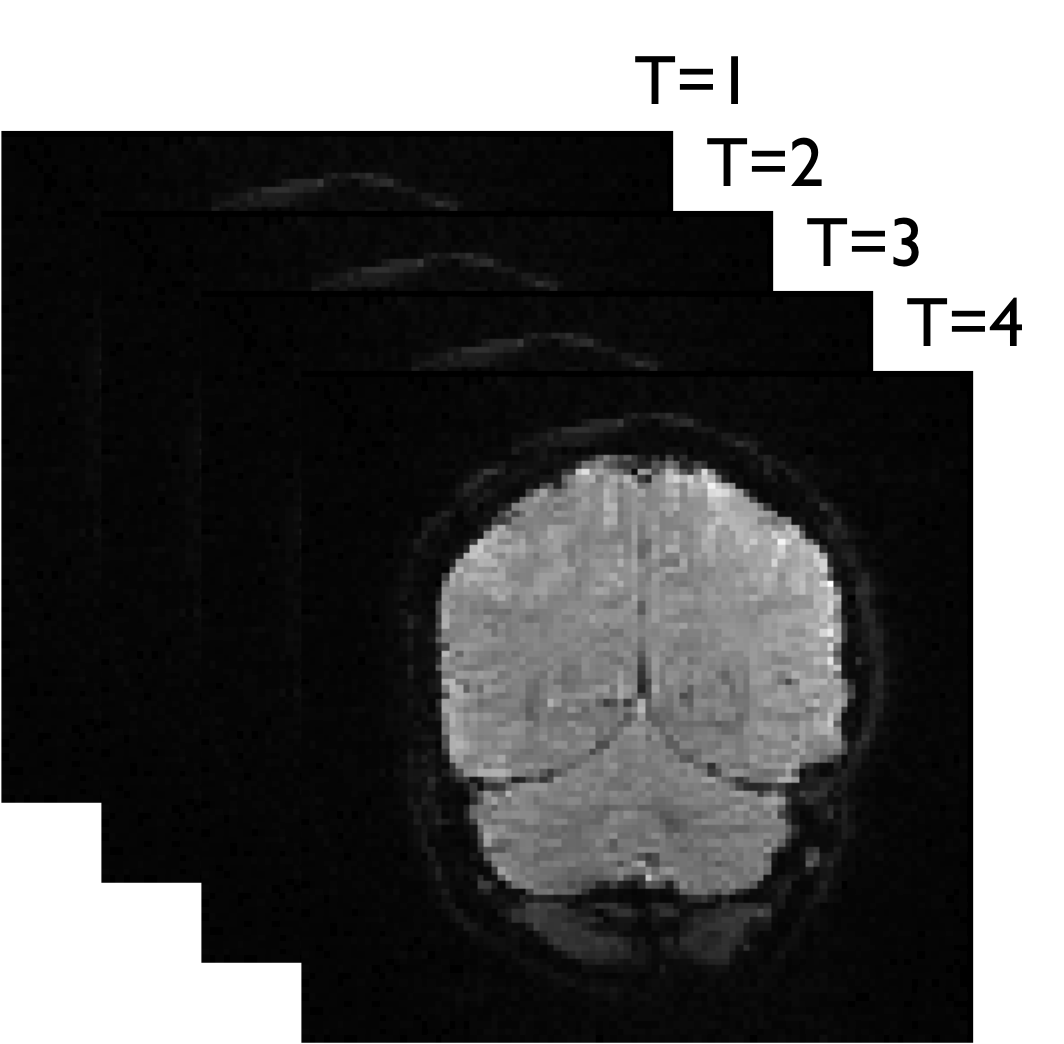
\includegraphics[height=5.7cm]{figures/t1_2_3_4}
\end{frame}

\begin{frame}
\frametitle{Time-series in fMRI data}
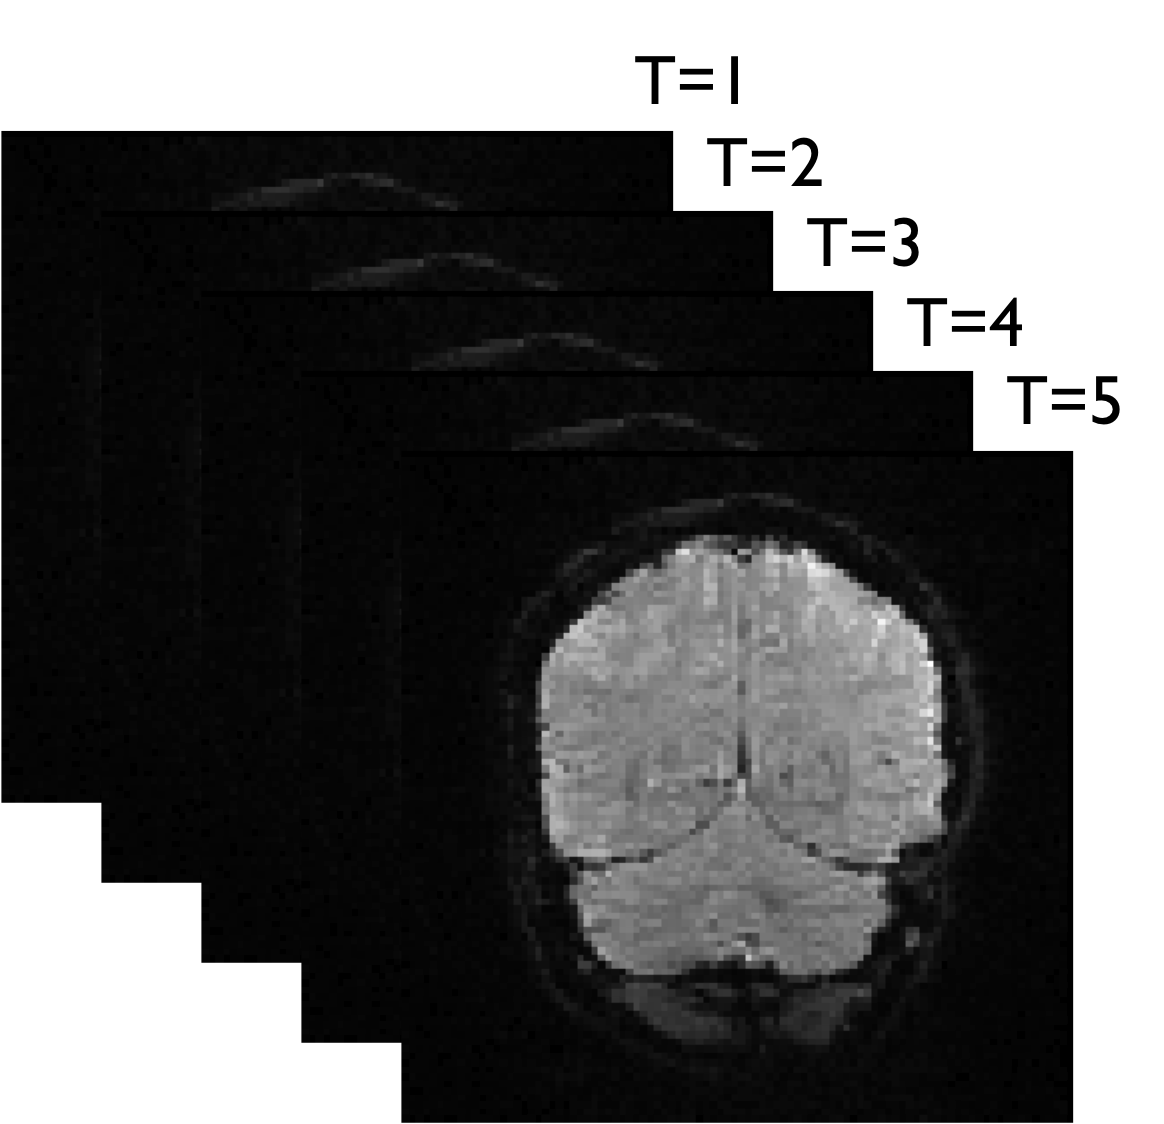
\includegraphics[height=5.7cm]{figures/t1_2_3_4_5}
\end{frame}

\begin{frame}
\frametitle{Time-series in fMRI data}
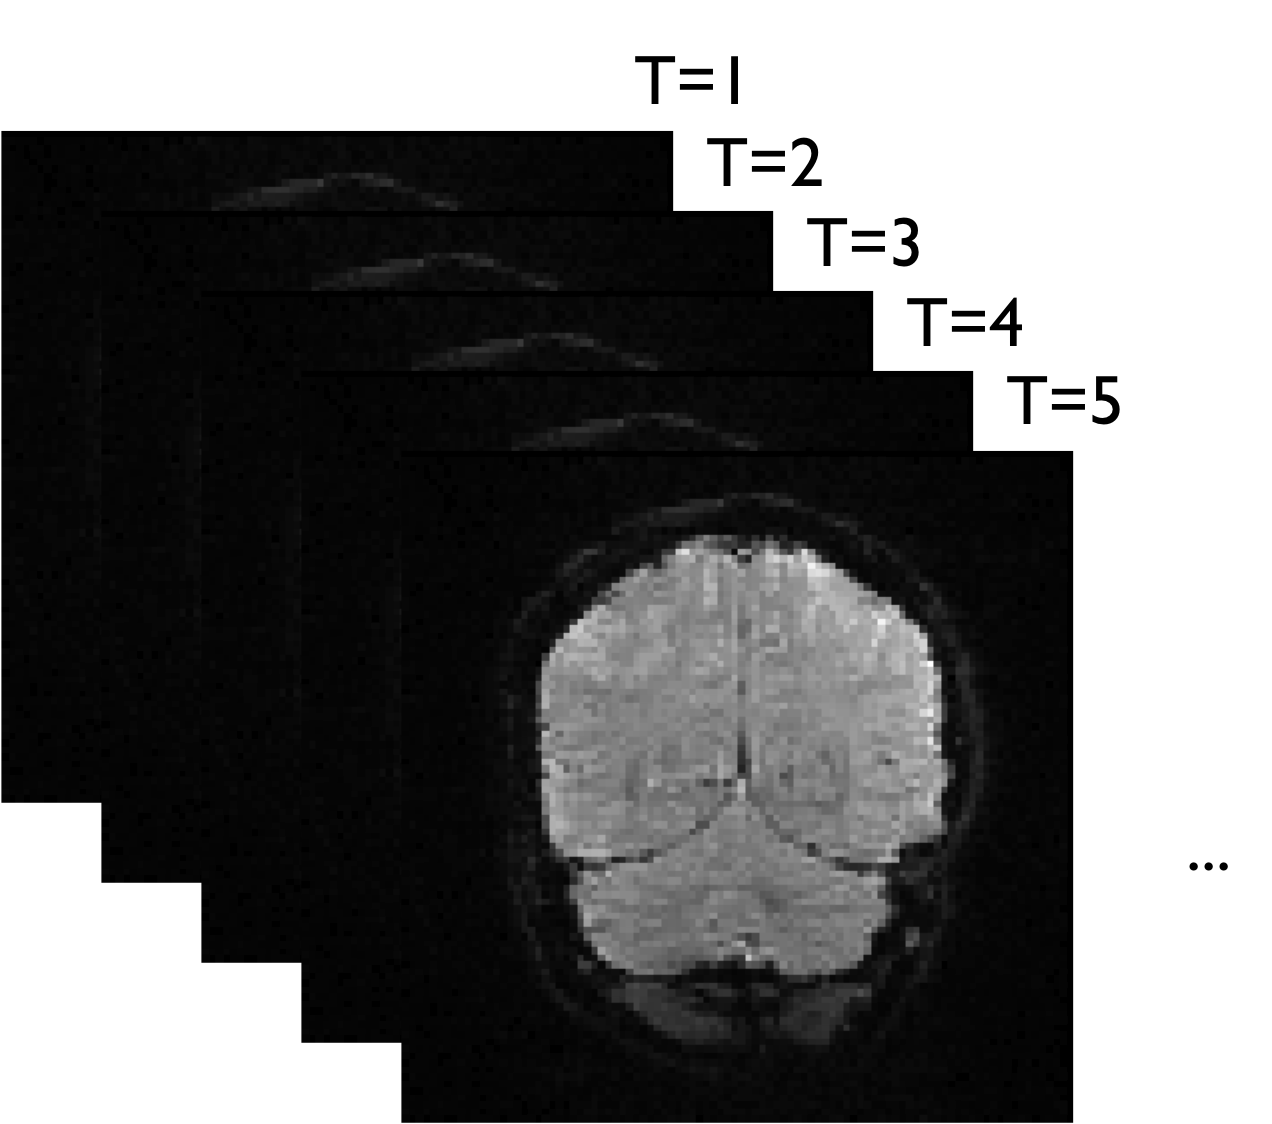
\includegraphics[height=5.7cm]{figures/t1_5_etc}
\end{frame}

\begin{frame}
\frametitle{Time-series in fMRI data}
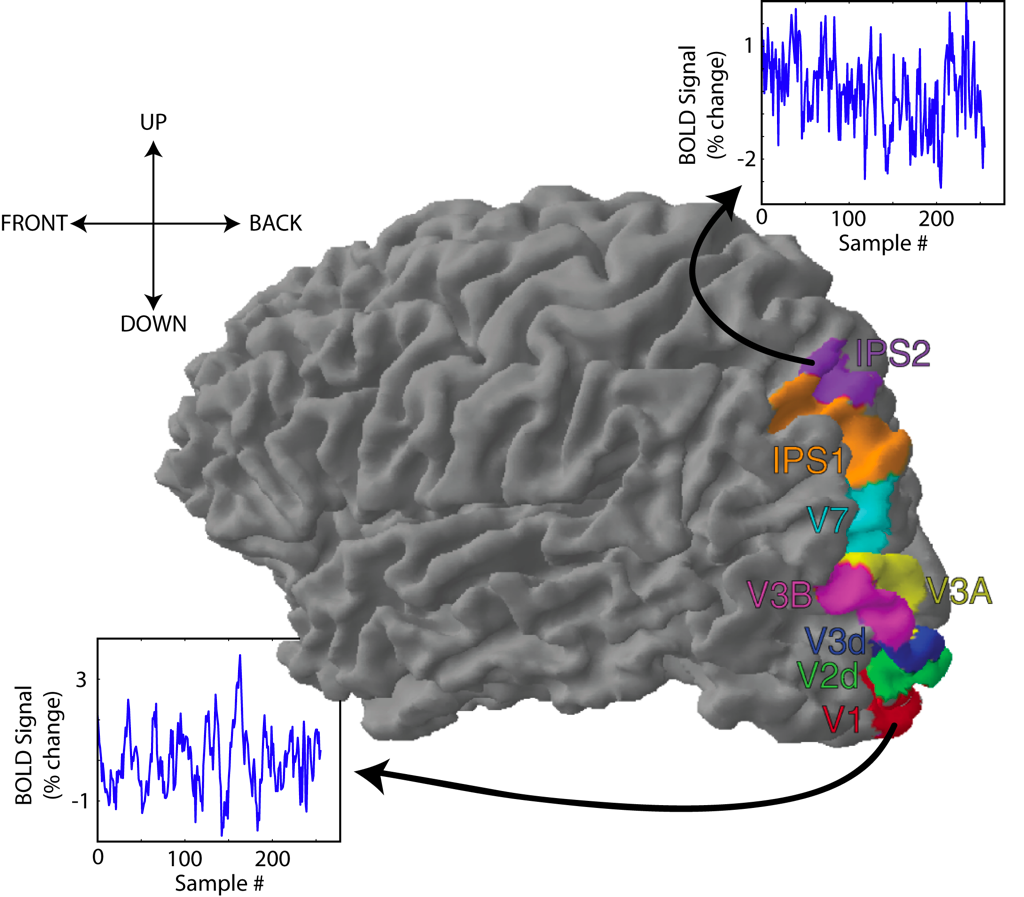
\includegraphics[height=5.7cm]{figures/brain_w_tseries}
\end{frame}


\begin{frame}
\frametitle{Levels of time-series analysis}
\begin{itemize}
\pause
\item
Univariate analysis: 
\pause
\item 
The analysis of the characteristics of the single time-series
\pause
\item
Example: event-related analysis
\end{itemize}
\end{frame}

\begin{frame}
\frametitle{Univariate analysis}
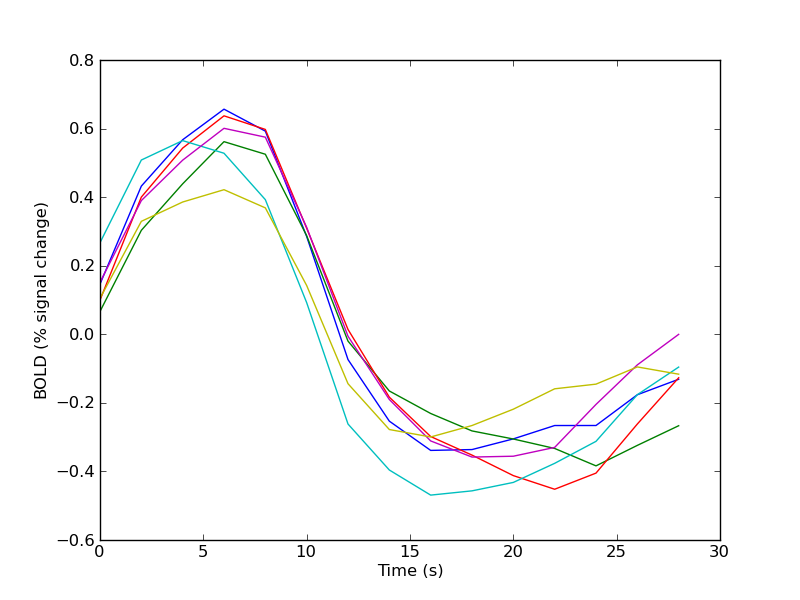
\includegraphics[height=5.7cm]{figures/event_related_fmri_02}
\end{frame}

\begin{frame}
\frametitle{Levels of time-series analysis}
\begin{itemize}
\item
Univariate analysis: 
\item 
The analysis of the characteristics of the single time-series
\pause
\item
Bivariate analysis:
\pause
\item
Relationships between pairs of time-series
\pause
\item
Example: Functional connectivity
\end{itemize}
\end{frame}

\begin{frame}
\frametitle{Functional connectivity}
What are the functional relations between different parts of the brain?
\end{frame}

\begin{frame}
\frametitle{Resting-state fMRI}
Functional connectivity at 'rest'
\end{frame}

\begin{frame}
\frametitle{Correlations}
\pause
Zero-order correlation:
\pause
$r_{xy} = \sum_{i=0}^{T}{\frac{(x_i-\hat{x})(y_i-\hat{y})}{\sigma_x \sigma_y}}$
\end{frame}

\begin{frame}
\frametitle{Resting state connectivity}
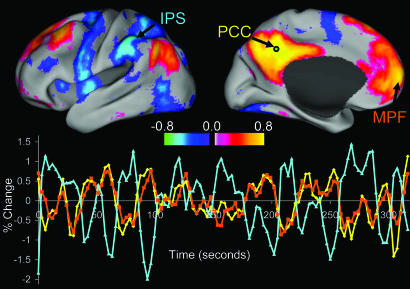
\includegraphics[height=5.7cm]{figures/fox_et_al}
\\
\hfill
Fox et al. (2005)
\end{frame}

\begin{frame}
\frametitle{What about the following time-series?}
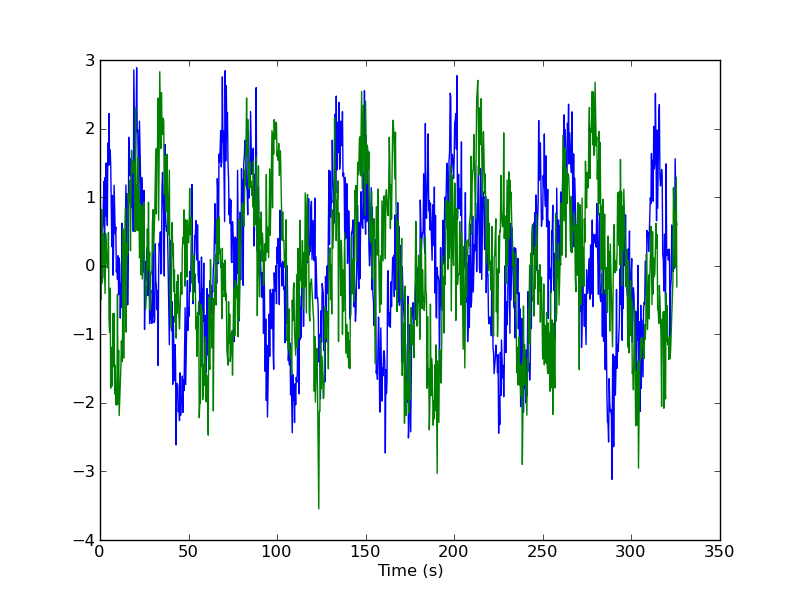
\includegraphics[height=5.7cm]{figures/outa_phase_tseries}
\end{frame}

\begin{frame}
\frametitle{Cross-correlation}
$Rxy(\tau) = \sum_{i=0}^{T}{x(t)y(t+\tau)}$
\end{frame}

\begin{frame}
\frametitle{Cross-correlation}
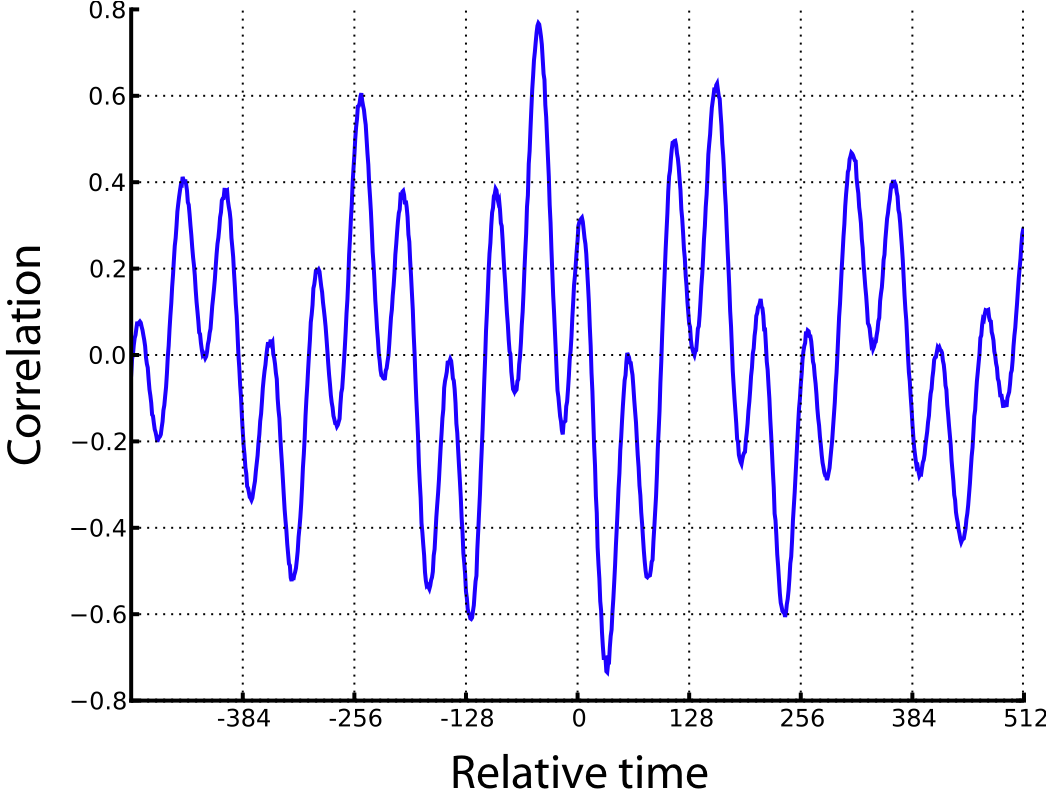
\includegraphics[height=5.7cm]{figures/outa_phase_xcorr}
\end{frame}

\begin{frame}
\frametitle{Cross-correlation}
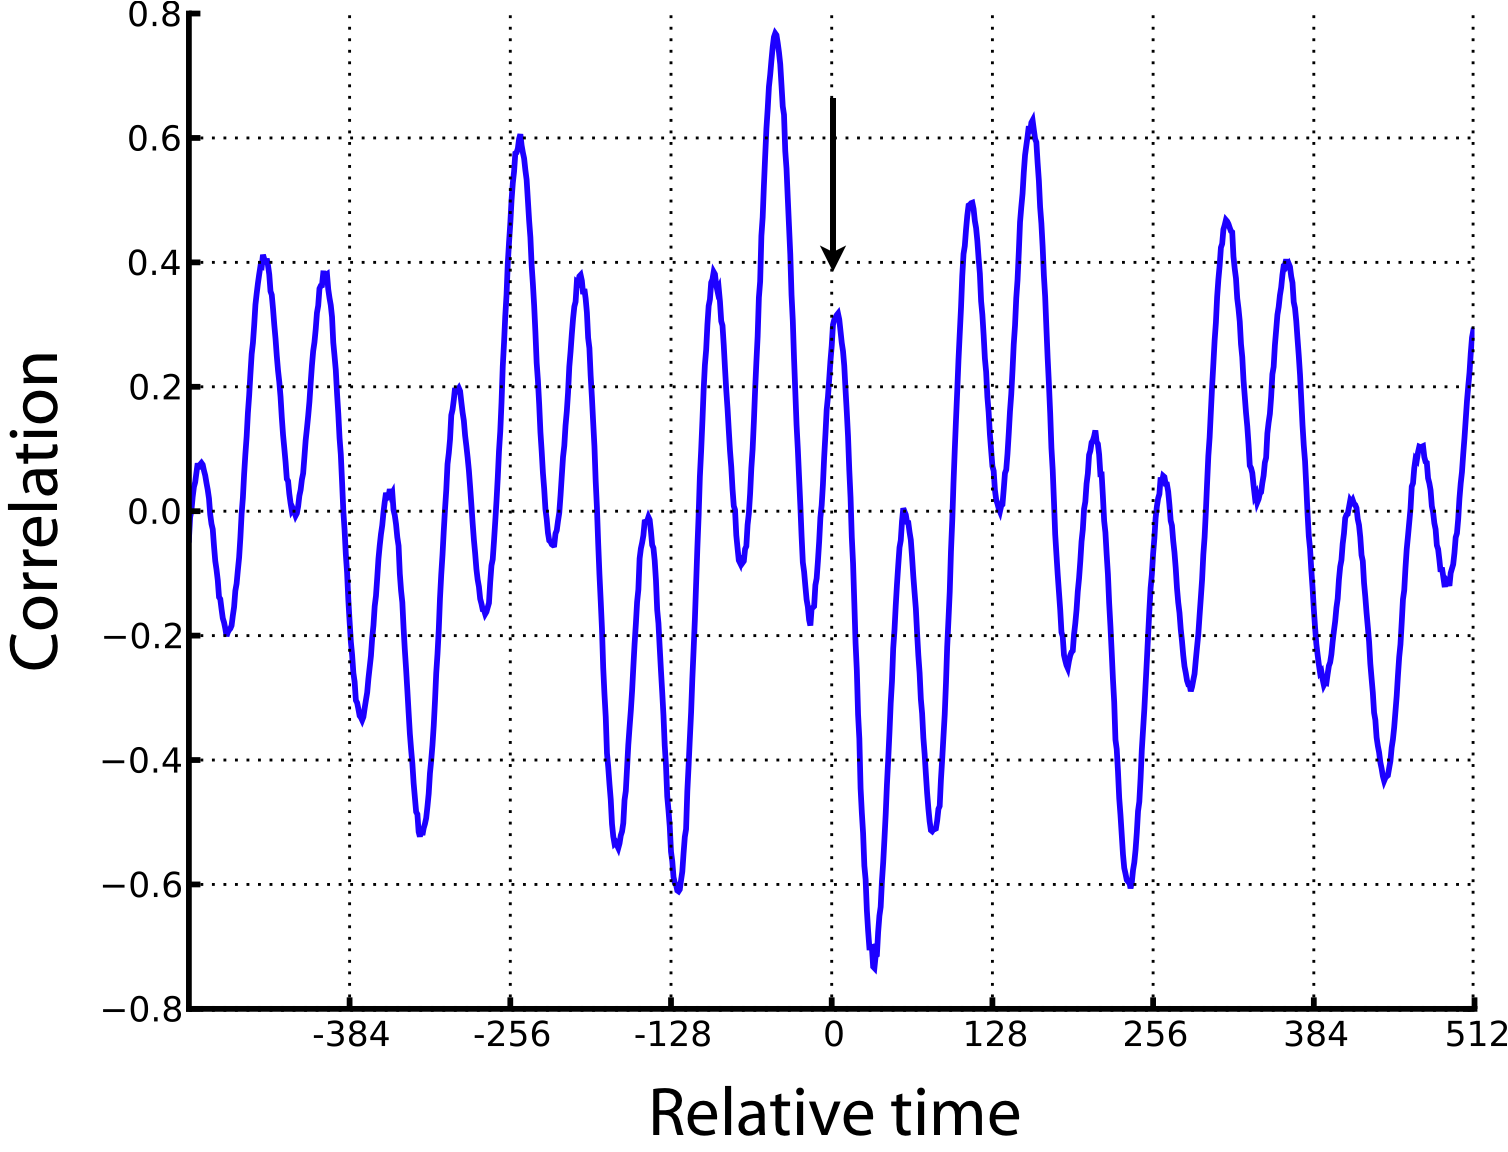
\includegraphics[height=5.7cm]{figures/outa_phase_xcorr_w_arrow}
\end{frame}

\begin{frame}
\frametitle{Cross-correlation}
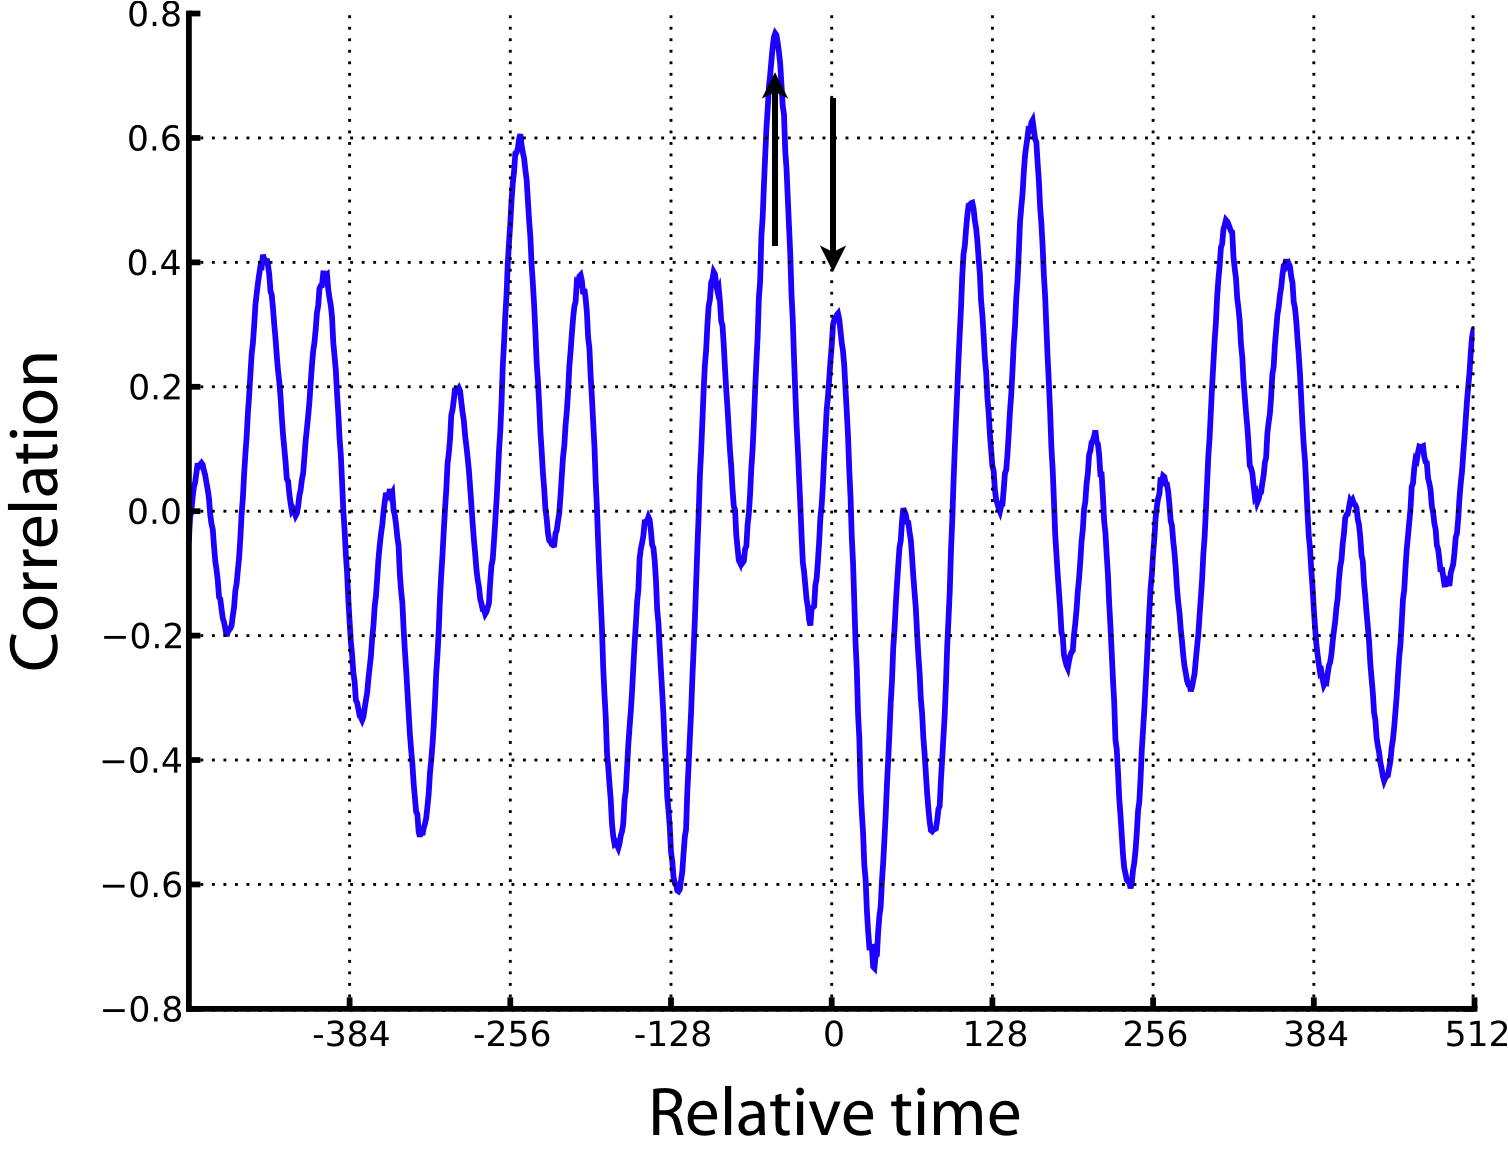
\includegraphics[height=5.7cm]{figures/outa_phase_xcorr_w_two_arrows}
\end{frame}

\begin{frame}
\frametitle{}
Why should we care? 
\end{frame}

\begin{frame}
\frametitle{Hemodynamic delays}
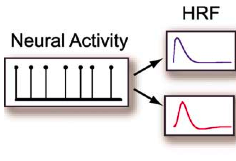
\includegraphics[height=2.7cm]{figures/hemo}
\end{frame}

\begin{frame}
\frametitle{Hemodynamic delays}
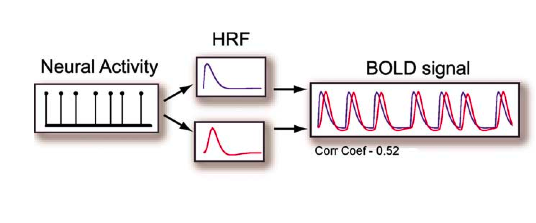
\includegraphics[height=3.7cm]{figures/tseries_w_hemo}
\end{frame}

\begin{frame}
\frametitle{Coherency}
A spectral analog of correlation
\end{frame}

\begin{frame}
\frametitle{Coherency}
$C_{xy}(\omega) = \frac{f_{xy}(\omega)}{f_{xx}(\omega)f_{yy}(\omega)}$
\pause
\\
\vfill
Where, $f_{xy}$ is the cross-spectral density and 
\\
$f_{xx}$ is the PSD of $x$
\end{frame}

\begin{frame}
\frametitle{Coherency}
Coherency is complex-valued:
\\
\pause
\vfill
Coherence: $Coh_{xy} (\omega) = abs(C_{xy}(\omega)) = $
\pause
$\frac{|f_{xy}(\omega)|}{f_{xx}(\omega)f_{yy}(\omega)}$
\vfill
\end{frame}

\begin{frame}
\frametitle{Coherency}
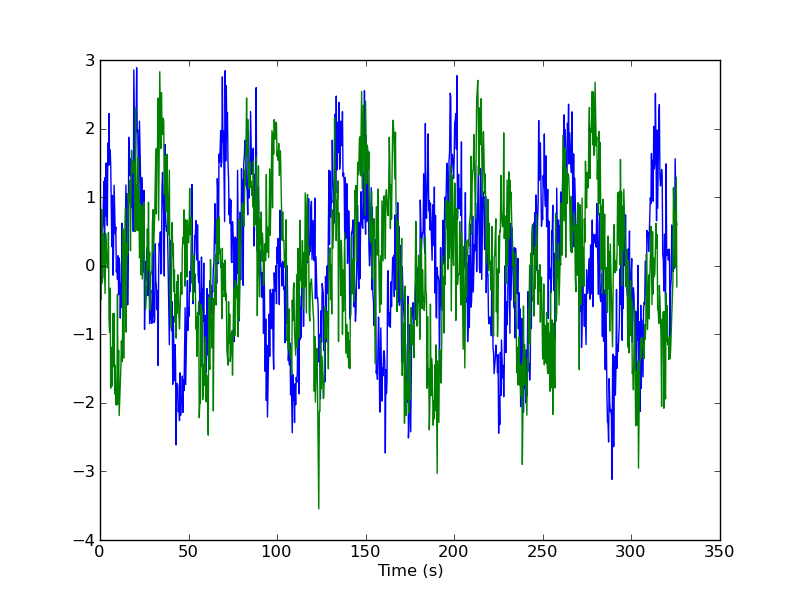
\includegraphics[height=5.7cm]{figures/outa_phase_tseries}
\end{frame}

\begin{frame}
\frametitle{Coherency}
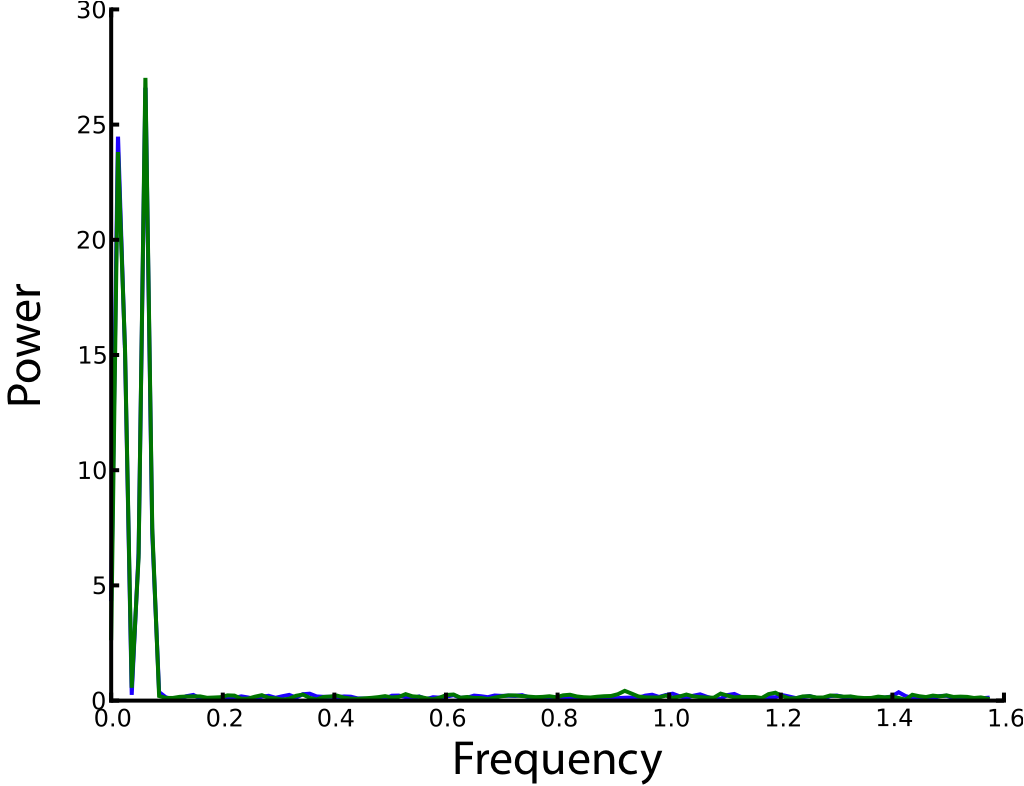
\includegraphics[height=5.7cm]{figures/outa_phase_tseries_psd}
\end{frame}

\begin{frame}
\frametitle{Coherence}
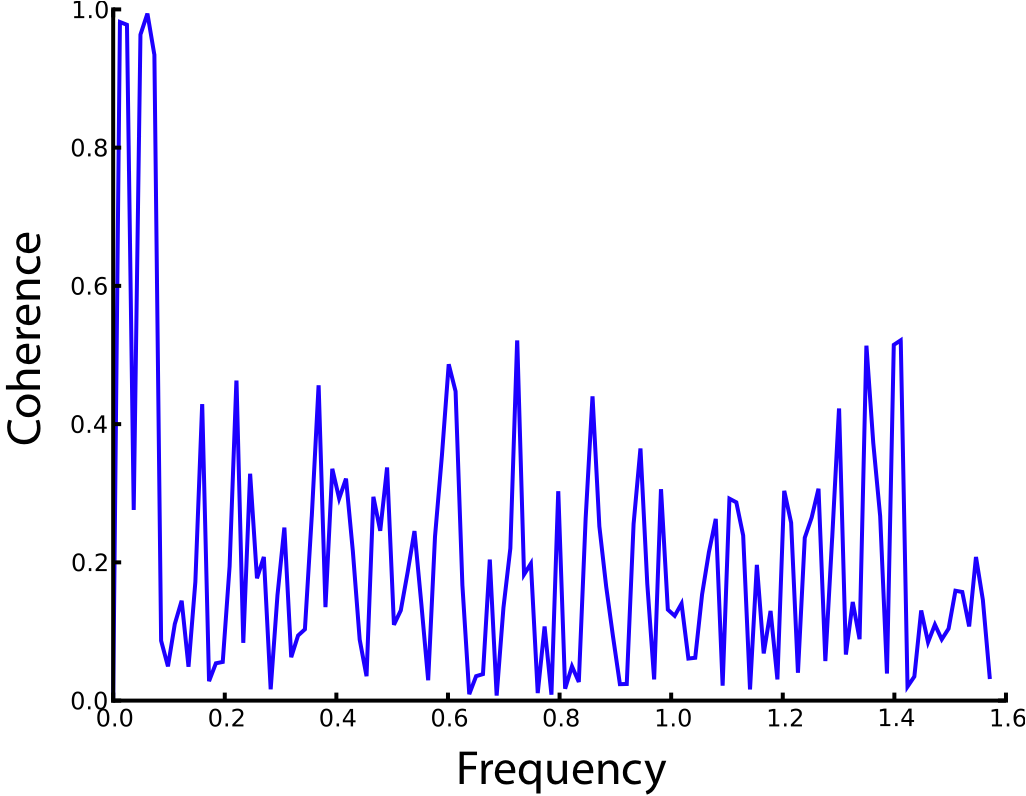
\includegraphics[height=5.7cm]{figures/outa_phase_tseries_coh}
\end{frame}

\begin{frame}
\frametitle{Coherency}
Coherency is complex-valued:
\\
\vfill
Coherence: $Coh_{xy} (\omega) = abs(C_{xy}(\omega)) = $
$\frac{|f_{xy}(\omega)|}{f_{xx}(\omega)f_{yy}(\omega)}$
\\
\pause
\vfill
Phase: $\phi(\omega)= angle(C_{xy}) = tan^{-1}\frac{\Im(f_{xy}(\omega))}{\Re(f_{xy}(\omega))}$
\end{frame}


\begin{frame}
\frametitle{Relative phase}
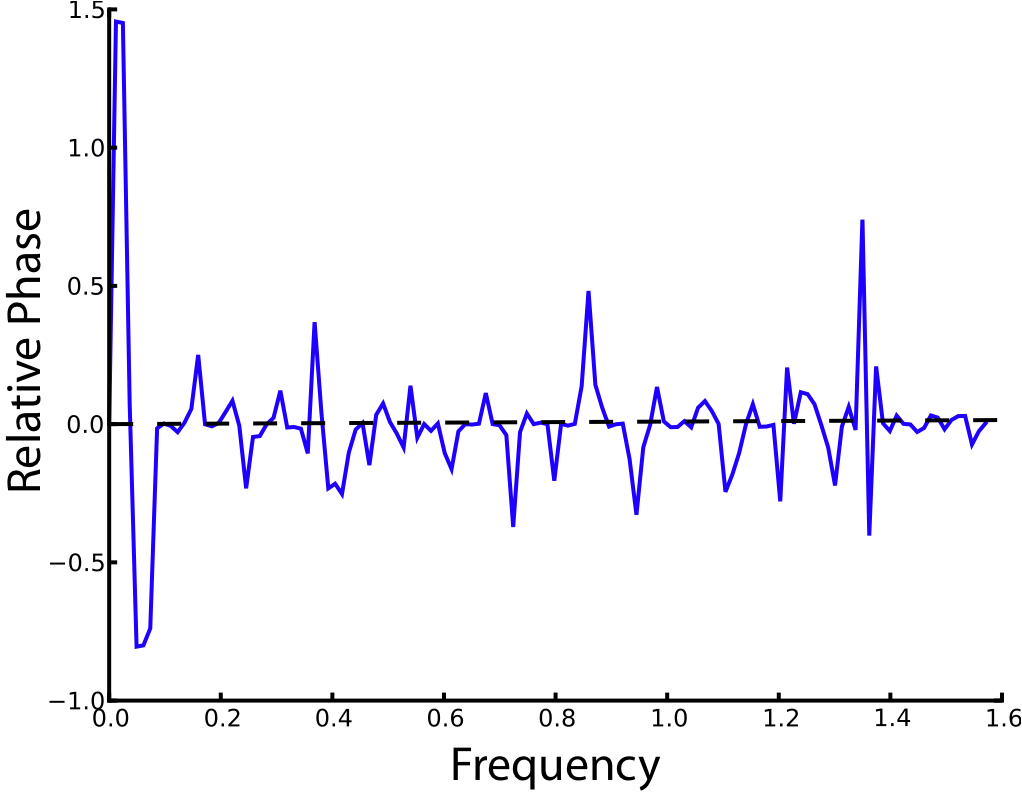
\includegraphics[height=5.7cm]{figures/outa_phase_tseries_ph}
\end{frame}

\begin{frame}
\frametitle{Coherency}
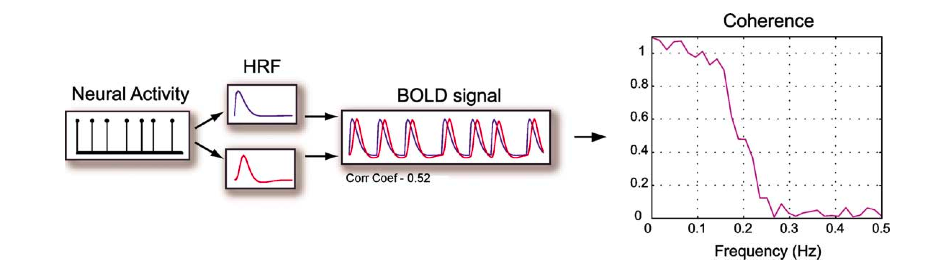
\includegraphics[height=2.7cm]{figures/tseries_w_hemo_w_coh}
\\
\hfill
Sun et al. (2004,2005)
\end{frame}

\begin{frame}
\frametitle{Using coherency to study task-related networks}
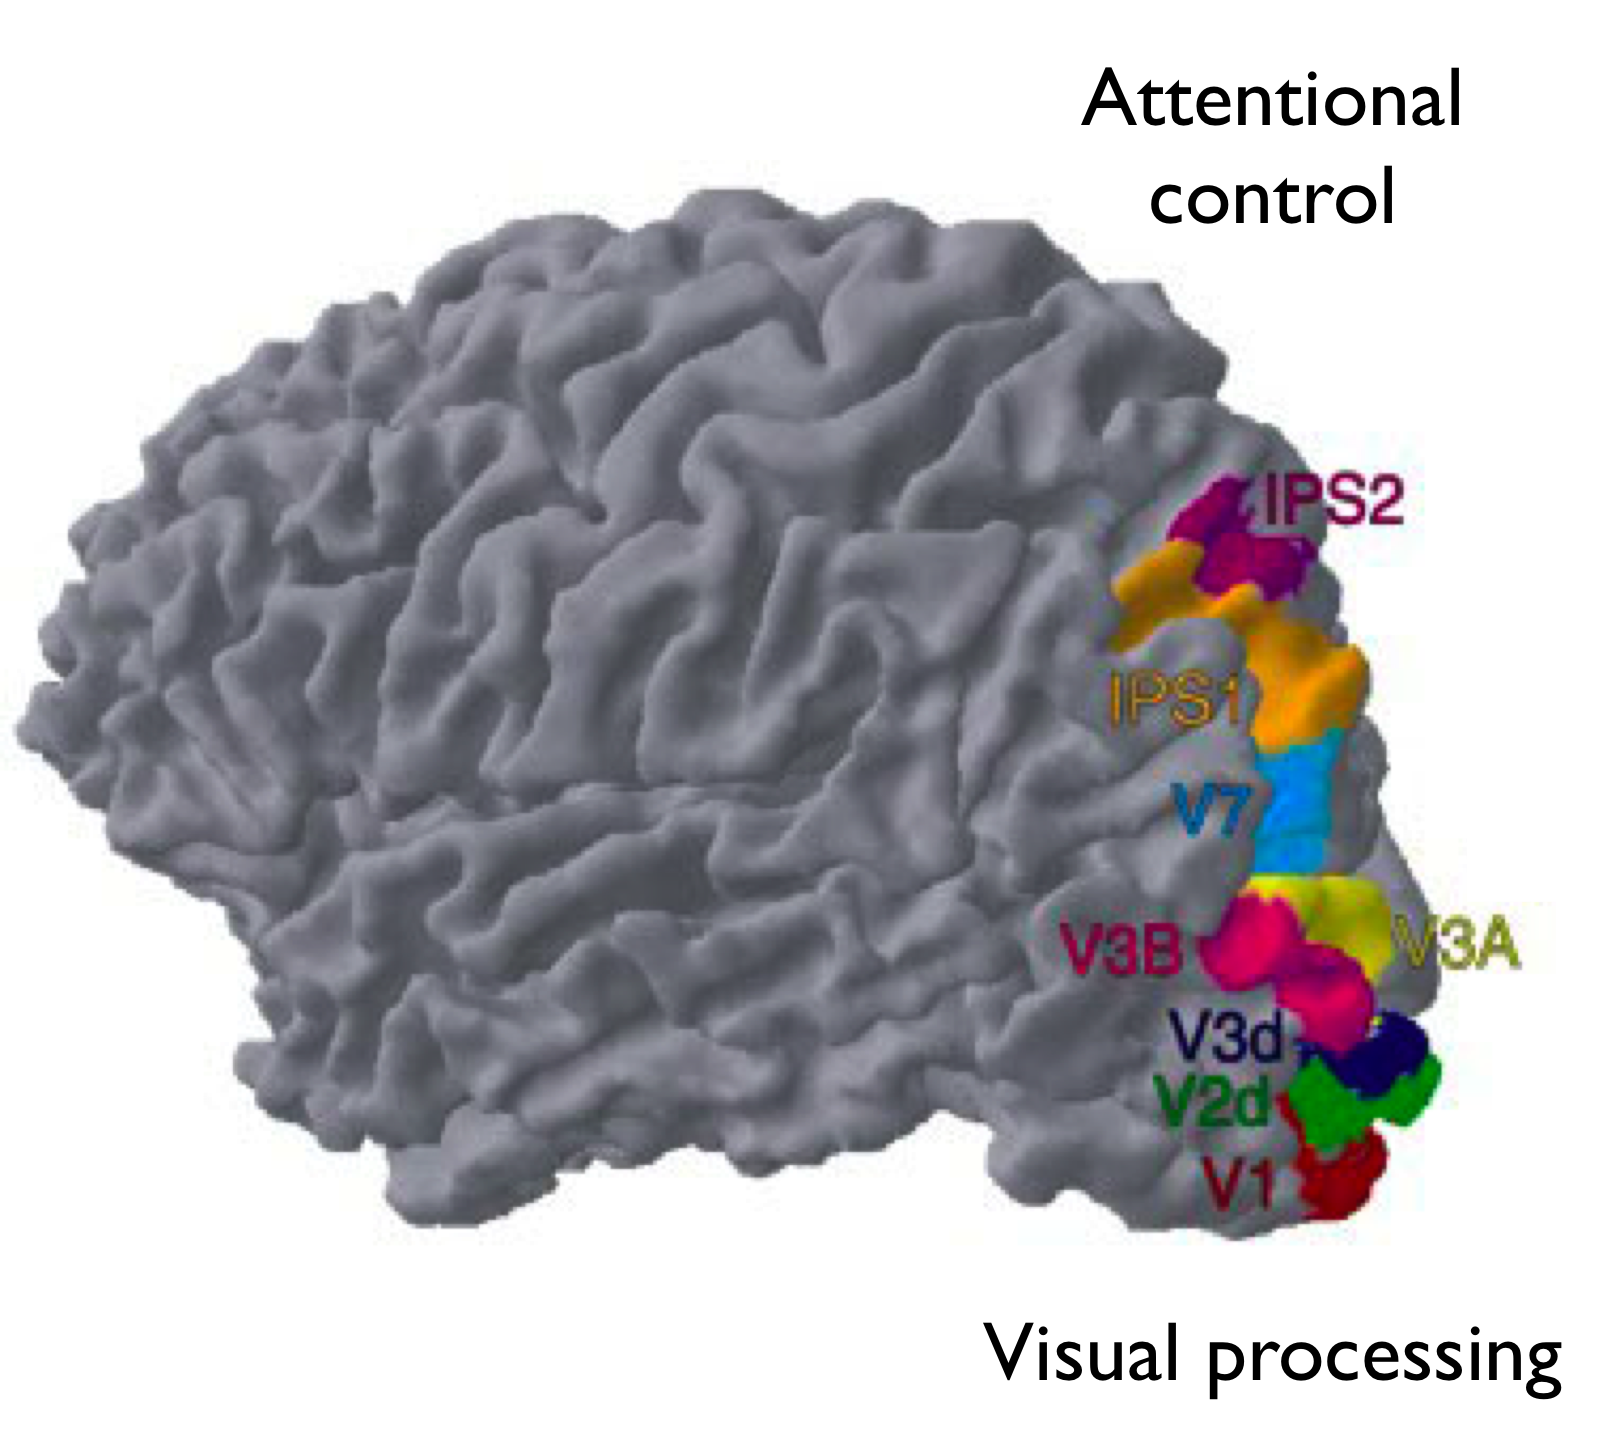
\includegraphics[height=5.7cm]{figures/lauritzen1}
\\
\hfill 
Lauritzen et al. (2009)
\end{frame}


\begin{frame}
\frametitle{Covert attention task}
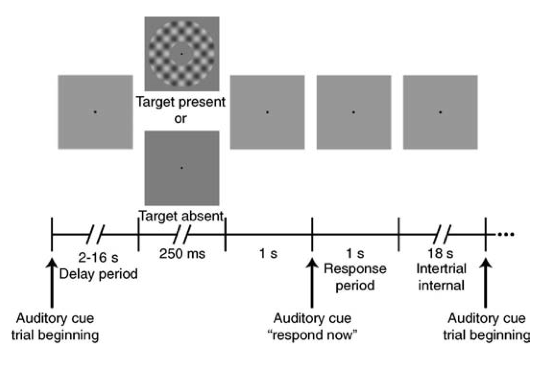
\includegraphics[height=5.7cm]{figures/lauritzen2}
\\
\hfill 
Lauritzen et al. (2009)
\end{frame}

\begin{frame}
\frametitle{Baseline coherence}
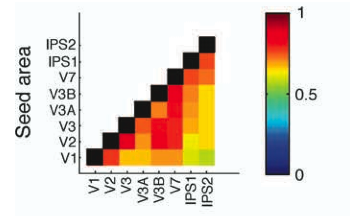
\includegraphics[height=2.7cm]{figures/lauritzen3}
\\
\hfill 
Lauritzen et al. (2009)
\end{frame}

\begin{frame}
\frametitle{Attention coherence}
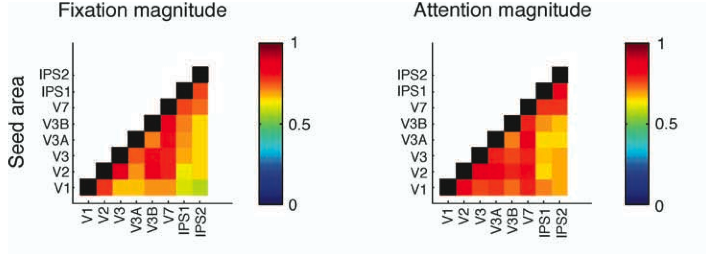
\includegraphics[height=2.7cm]{figures/lauritzen4}
\\
\hfill 
Lauritzen et al. (2009)
\end{frame}

\begin{frame}
\frametitle{Difference in coherence}
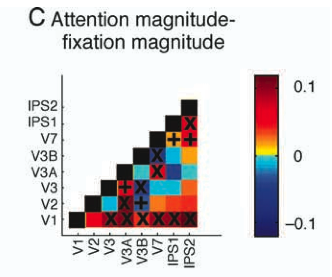
\includegraphics[height=5.7cm]{figures/lauritzen5}
\\
\hfill 
Lauritzen et al. (2009)
\end{frame}


\begin{frame}
\frametitle{Time delay}
The time-delay between two time-series can be calculated from the phase delay 
\\ 
\pause
\vspace{1cm}
$\Delta t (\omega) = \frac{\phi(\omega)}{2 \pi \omega}$
\end{frame}

\begin{frame}
\frametitle{Time delay}
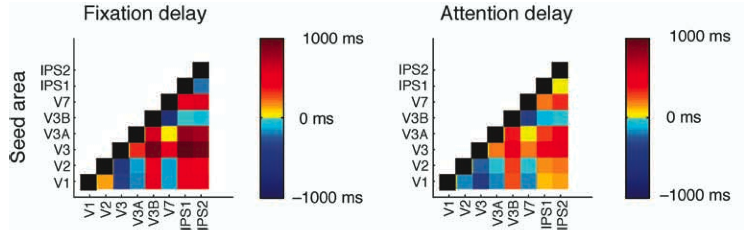
\includegraphics[height=2.7cm]{figures/lauritzen6}
\\
\hfill 
Lauritzen et al. (2009)
\end{frame}

\begin{frame}
\frametitle{Delay difference}
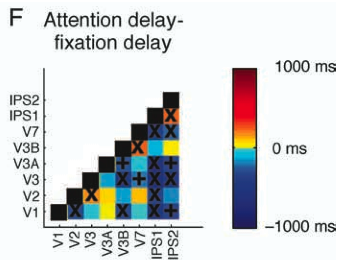
\includegraphics[height=5.7cm]{figures/lauritzen7}
\\
\hfill 
Lauritzen et al. (2009)
\end{frame}

\begin{frame}
\frametitle{Task-related network changes:}
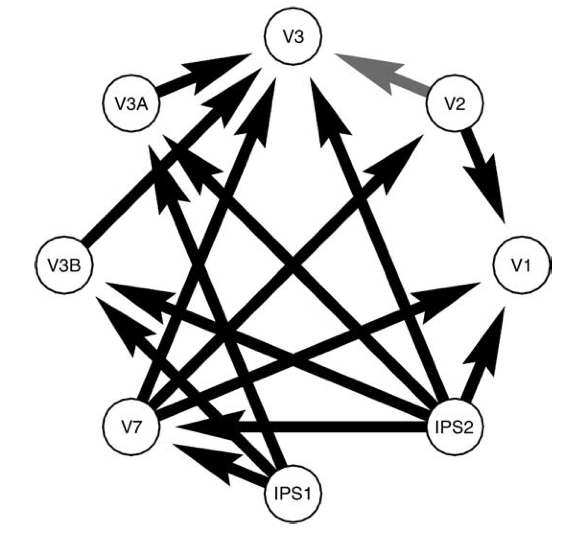
\includegraphics[height=5.7cm]{figures/lauritzen8}
\\
\hfill 
Lauritzen et al. (2009)
\end{frame}

\begin{frame}
\frametitle{Coherency analysis: summary}
\pause
\begin{itemize}
\item
Coherency analysis is a spectral analog of correlation
\pause
\item 
Not sensitive to relative delays
\pause
\item
When used for fMRI need to pay attention to: 
\pause
\item  
Baseline connectivity
\pause
\item
Defining a proper control condition
\end{itemize}

\end{frame}

\begin{frame}
\frametitle{\tt{Nitime}}
\begin{itemize}
\pause
\item
Software library for the analysis of time-series from neuroscience data
\pause
\item
Written in Python
\pause
\item 
Free and open source (no black-boxes involved!)
\item
\pause
\tt{http://nipy.org/nitime}
\end{itemize}
\end{frame}


\begin{frame}
\frametitle{\tt{Nitime} components:}
\begin{itemize}
\pause
\item
\tt{nitime.timeseries}
\pause
\item
\tt{nitime.viz}
\pause
\item
\tt{nitime.algorithms}
\pause
\item
\tt{nitime.analysis}
\pause 
\item
\tt{nitime.utils}
\end{itemize}
\end{frame}

\begin{frame}[fragile]
\frametitle{Simple example:}
\pause
\begin{lstlisting}
>>> import nitime.timeseries as ts 
>>> t1 = ts.TimeSeries(data=[1,2,3,4],
                       sampling_interval=1.5,
                       time_unit='s')
\end{lstlisting}
\pause
\begin{lstlisting}
>>> t1.time
UniformTime([ 0. ,  1.5,  3. ,  4.5], 
                       time_unit='s')
\end{lstlisting}

\pause
\begin{lstlisting}
>>> t1.sampling_rate
0.666666666667 Hz
\end{lstlisting}
\end{frame}

\begin{frame}[fragile]
\frametitle{Vizualization}
\pause
\begin{lstlisting}
>>> import nitime.viz as viz
>>> viz.plot_tseries(t1)
\end{lstlisting}
\end{frame}

\begin{frame}
\frametitle{Vizualization}
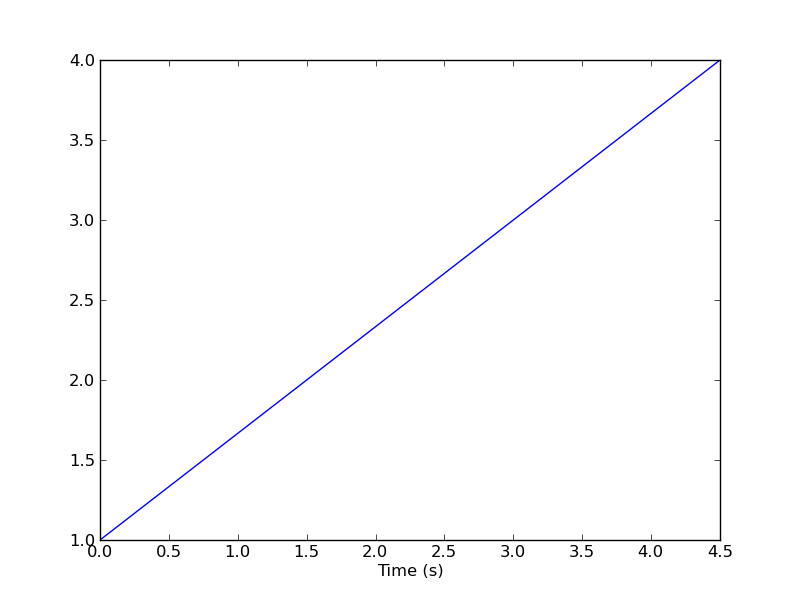
\includegraphics[height=5.7cm]{figures/simple_viz}
\end{frame}

\begin{frame}[fragile]
\frametitle{Vizualization}
\begin{lstlisting}
>>> t2 = ts.TimeSeries(data=[1,2,3,4],
                       sampling_interval=1.5,
                       time_unit='ms')
>>> viz.plot_tseries(t2)
\end{lstlisting}
\end{frame}

\begin{frame}
\frametitle{Vizualization}
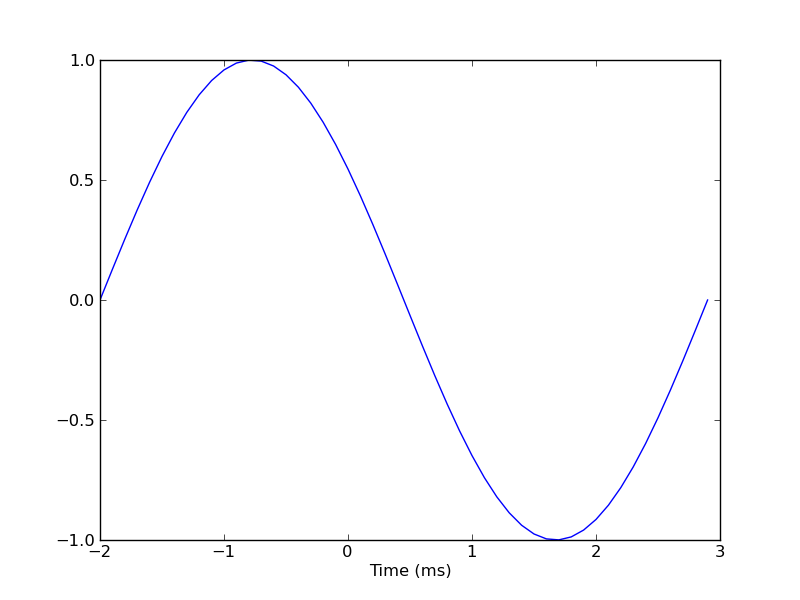
\includegraphics[height=5.7cm]{figures/simple_viz2}
\end{frame}

\begin{frame}
\frametitle{\tt{nitime.algorithms}}
\begin{itemize}
\pause
\item
coherence
\pause
\item
event-related 
\pause
\item
filter
\pause
\item
spectral
\item
\pause
autoregressive
\end{itemize}
\end{frame}

\begin{frame}[fragile]
\frametitle{Example: spectral analysis of an autoregressive process}
Autoregressive processes are of the form: 
\pause
$x(t) = a_1x(n-1) + a_2x(t-2) + ... + a_ix(t-i) + \epsilon_x$
\\
\pause
We generate a 2nd order AR: 
\\
\pause
\begin{lstlisting}
>>> import nitime.utils as utils 
\end{lstlisting}
\begin{lstlisting}
>>> ar2,n,c = utils.ar_generator(
         coefs=[0.1, -0.2], N=2**16)
\end{lstlisting}
\end{frame}

\begin{frame}[fragile]
\frametitle{Example: spectral analysis of an autoregressive process}
We perform a spectral analysis:
\begin{lstlisting}
>>> import nitime.algorithms as alg
>>> f, c = alg.get_spectra(ar2)
>>> import matplotlib.pylab as pl 
>>> pl.plot(f, c)
\end{lstlisting}
\end{frame}

\begin{frame}
\frametitle{Vizualization}
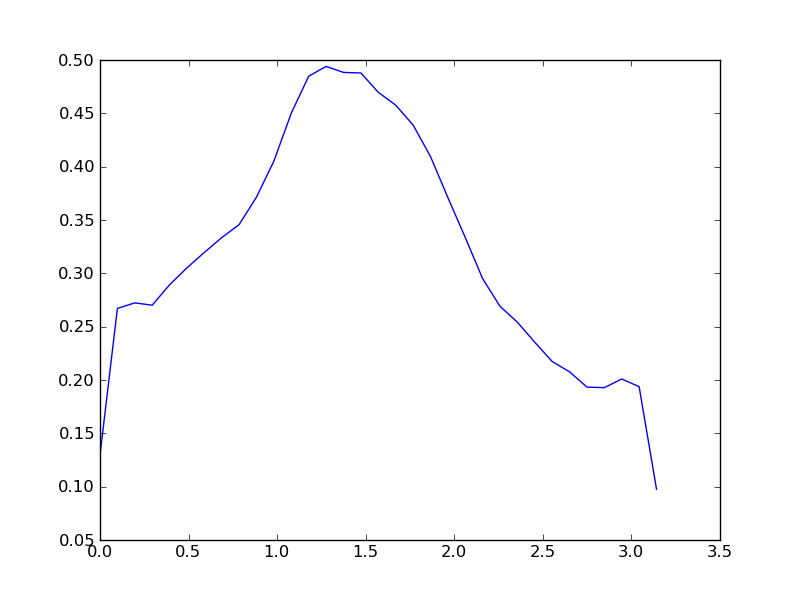
\includegraphics[height=5.7cm]{figures/ar_spectrum}
\end{frame}


\begin{frame}
\frametitle{\tt{nitime.analysis}}
\begin{itemize}
\pause
\item
coherence
\pause
\item
event-related 
\pause
\item
filter
\pause
\item
spectral
\item
\pause
autoregressive
\end{itemize}
\end{frame}

\end{document}
